\documentclass{siamltex}
\usepackage{xeCJK}
\usepackage{amsmath}

\usepackage{color}
\usepackage{amsfonts,amsmath}
\usepackage{graphicx}
\usepackage{tikz}
\usepackage[algosection,vlined,ruled,linesnumbered]{algorithm2e}
\usepackage{subfigure}
\usepackage{booktabs}
\usepackage{wasysym}
\usepackage{multirow}
\newcommand{\commentKK}[1]{{\color{red!80!yellow}{#1}}}
\newcommand{\commentBL}[1]{{\color{blue!80!white}{#1}}}
\newcommand{\commentMR}[1]{{\color{red!50!blue}{#1}}}
\newcommand{\commentAF}[1]{{\color{red!95}{#1}}}
\newcommand{\alert}[1]{{\textbf{\color{red}{#1}}}}
\newcommand{\sign}{{\rm sign}}
\newcommand{\Dslash}{\mathcal{D}}
\newcommand{\range}{\mathop{\mathrm{range}}\nolimits}
\newcommand{\myspan}{\mbox{span}}
\newcommand{\kernel}{\mathop{\mathrm{kern}}\nolimits}
\newcommand{\MSAP}[1]{M_\mathit{SAP}^{(#1)}}
\newcommand{\MSAPone}{M_\mathit{SAP}}
\newcommand{\ESAP}{E_\mathit{SAP}}
\newcommand{\ddml}[2]{DDML($#1,#2$)}
\newcommand{\ddmlsetup}[2]{DDMLsetup($#1,#2$)}
\newcommand{\ncy}{n_\mathit{cy}}
\newcommand{\ninv}{n_\mathit{inv}}
\newcounter{confcounter}
\newcommand{\conflabel}[1]{\refstepcounter{confcounter} \label{#1}}
\DontPrintSemicolon
\setcounter{topnumber}{5}
\renewcommand*\topfraction{.85}
\setcounter{bottomnumber}{5}
\renewcommand*\bottomfraction{.7}
\setcounter{totalnumber}{10}
\renewcommand*\textfraction{.15}
\renewcommand*\floatpagefraction{0.8}
\title{基于自适应聚合的格点威尔逊狄拉克算子域分解多重网格  \thanks{This work was partially funded by Deutsche Forschungsgemeinschaft (DFG) Transregional Collaborative Research Centre 55 (SFB/TRR55)}   }
\author{A. Frommer\thanks{Department of Mathematics, Bergische Universit\"{a}t Wuppertal, 42097 Germany, {\tt  \{ frommer,kkahl,leder,rottmann \} @math.uni-wuppertal.de}.}
\and K. Kahl\footnotemark[2]
\and S. Krieg\thanks{Department of Physics, Bergische Universit\"{a}t Wuppertal, 42097 Germany and J\"{u}lich Supercomputing Centre, Forschungszentrum J\"{u}lich, 52428 J\"{u}lich, Germany, {\tt s.krieg@fz-juelich.de}.}
\and B. Leder\footnotemark[2]
\and M. Rottmann\footnotemark[2]
}
\begin{document}
\maketitle
\begin{abstract}在格点 QCD 计算中,大量的工作都花在求解离散化的狄拉克方程上。传统的 Krylov 求解器在系统规模较大和物理上有趣的参数区域时会表现出显著的减速。我们提出了一种域分解自适应代数多重网格法,将其用作预处理器来求解狄拉克方程的“三叶草改进”威尔逊离散化。这种方法结合并改进了两种方法,即域分解和自适应代数多重网格,这两种方法以前在格点 QCD 中分别使用过。我们在使用并行生产代码实现进行的大量数值测试中表明,与传统的 Krylov 子空间方法、域分解方法和其他分层方法相比,这种方法可以实现显著的加速,适用于实际的系统规模。  \end{abstract}

\begin{keywords}
  multilevel, multigrid, lattice QCD, Wilson Dirac operator, domain decomposition, aggregation, adaptivity, parallel computing.
\end{keywords}

\begin{AMS}
  65F08,
  65F10,
  65Z05,
  65Y05
\end{AMS}
\section{介绍  }    格点 QCD 模拟是世界上最难计算的问题之一,当今超级计算机资源的很大一部分都花在这些模拟上    \cite{PRACE:ScAnnRep12,PRACE:ScC12}    。我们在本文中关注三个方面:我们希望使与 QCD 和格点 QCD 相关的数学建模在科学计算界更受欢迎,因此花了一些精力来解释基础知识。最重要的是,我们开发了一种新的、高效的自适应代数多重网格方法来解决具有离散化狄拉克算子的系统,并且我们基于先进的、生产代码质量实现和最新的物理数据展示了大量数值实验的结果。

格点 QCD 计算中的计算挑战在于反复求解非常大的稀疏线性系统
\begin{equation}\label{eq:discreteDirac}
  Dz = b,
\end{equation}    其中    $D = D(U,m)$    是四维时空格点上狄拉克算子的离散化,通常是威尔逊离散化。威尔逊狄拉克算子依赖于规范场    $U$    和质量常数    $m$    。最近,已经使用了具有最多    $144\times64^3$    个格点的格点,涉及求解具有    $452,\!984,\!832$    个未知数    \cite{Alexandrou:2011db,Bae:2011ff,Bali:2012qs,Durr:2010aw,Fritzsch:2012wq}    的线性系统。通常这些线性系统通过标准 Krylov 子空间方法求解。当接近物理相关参数值(即物理质量常数和格点间距    $a\rightarrow 0$    )时,它们的迭代次数会大大增加,这种现象在物理学文献中称为“临界减速”。因此,开发能够克服这些扩展问题的预处理器至关重要。目前最常见的预处理器是奇偶预处理器~    \cite{Degrand1990211,Lippert19991357}    、紧缩预处理器~    \cite{Luescher2007}    和域分解~    \cite{Nobile2012,Luescher2003}    。虽然这些方法比未预处理器版本的速度有显著提升,但它们的缩放行为没有改变,仍然会出现严重的减速。

格点 QCD 社区也在考虑多重网格方法,其动机是它们具有与格点间距无关的收敛潜力(例如,对于椭圆 PDE)。然而,由于所涉及的规范场的随机性,过去二十年来,仅基于底层 PDE 的多重网格方法处理格点狄拉克方程一直难以实现~    \cite{Ben-Av:1990gb,Brower:1987dd,Kalkreuter:1994fz,Vink:1991fa}    。随着自适应代数多重网格方法的出现,近年来可以构建用于 QCD 计算的有效预处理器。   \cite{MGClark2009, MGClark2010_1, MGClark2007, MGClark2010_2}    的开创性工作显示出非常有希望的结果。在那里,一种基于~    \cite{Brezina2005}    的自适应非平滑聚合方法已被提出用于解决 Wilson Dirac 系统。其实现作为 QOPQDP 包~    \cite{wwwQOPQDP}    的一部分向公众开放。

在物理学界,另一种分层技术,即最近提出的域分解类型求解器不精确紧缩,在    \cite{Luescher2007}    中开发,被广泛使用。此求解器的一个经过优化的代码已公开~    \cite{wwwDDHMC}    。不精确紧缩也可以看作是一种自适应方法。它执行一个设置阶段,允许构建一个较小的系统,即小狄拉克算子,然后将其用作高效预处理器的一部分。虽然不精确紧缩与    \cite{Brezina2005}    中的基于聚合的多重网格方法有着密切的联系,但它似乎是完全独立开发出来的。因此,不精确紧缩方法在成分排列方式上与典型的多重网格方法并不相似。特别是,它要求在每次迭代中对小狄拉克系统进行高精度求解。

在本文中,我们提出了一种多重网格法,它结合了    \cite{Luescher2007}    的各个方面(即域分解平滑器)和非平滑聚合(如    \cite{MGClark2010_1, MGClark2010_2}   )。我们的方法详细阐述了    \cite{MGClark2010_1, MGClark2010_2}    中的多重网格法,因为我们使用域分解法作为平滑器,而不是之前使用的 Krylov 子空间平滑器。这允许在混合架构上实现自然而高效的并行化。此外,我们大大改进了    \cite{MGClark2010_1, MGClark2010_2}    和    \cite{Luescher2007}    中的自适应设置,因为计算高效多重网格法所需的运算符层次所需的时间更少。我们的方法也可以看作是将    \cite{Luescher2007}    中的域分解技术转变为真正的多重网格法。现在只需要以较低的精度求解“小狄拉克”系统。尤其是,这允许以递归方式应用该方法,从而为更高效的  {    \em    多   }  网格方法(而不仅仅是双网格方法)开辟了道路。使用不精确的压缩方法,这是不可能的。

本文的结构如下。在    \ref{qcd_section}    节中,我们为非专业人士介绍了格点 QCD,并在此背景下介绍了域分解 Schwarz 方法。在    \ref{section:AMG}    节中,我们首先概述了代数多重网格方法,然后重点介绍了基于聚合的方法。因此,我们讨论了格点 QCD 的特性,并解释了构建多重网格层次结构的不同可能的自适应策略。在    \ref{sec:PID}    节中讨论了    \cite{Luescher2007}    中的不精确压缩方法,其中我们特别指出了与多重网格方法的不同之处,并描述了其设置的自适应性。在    \ref{sec:DDML}    节中,我们最终制定了多重网格方法,并在    \ref{sec:NR}    节中对其进行了详尽的数值测试。
\section{格点量子色动力学  }       \label{qcd_section}    量子色动力学 (QCD) 或强相互作用理论是四维时空中的量子场论,是基本粒子物理学标准模型的一部分。它具有很高的预测能力,即自由参数数量少。可以从该理论推导出的预测包括强子的质量、受强相互作用约束的复合粒子(例如核子、介子;参见~    \cite{Durr21112008}   )。强子的质量和许多其他预测必须非微扰地获得,即通过需要对理论进行离散化和数值评估的数值模拟。在简要描述连续 QCD 的相关方面之后,我们介绍了它在超立方晶格上的离散化,并讨论了使用迭代(Krylov 子空间)方法解决出现的线性方程组的必要性。由于它们的病态性质,建议进行预处理,并讨论使用域分解方法作为多重网格构建的先决条件。
\subsection{连续量子色动力学  }       \label{continuum_qcd}    对 QCD 作为量子场论的详细描述超出了本文的范围。我们只是向读者介绍理解格点离散化所必需的重要概念和符号。

QCD 的自由度是物质场(称为夸克)和规范场(称为胶子)。格点 QCD 数值方法的核心是离散化的连续狄拉克方程    \begin{equation}\label{Dirac_eq}
  (\Dslash+m)\psi = \eta
\end{equation}   ,该方程描述了给定胶子场背景下夸克的动力学以及夸克和胶子的相互作用。这里,   $\psi = \psi(x)$    和    $\eta = \eta(x)$    表示物质场。它们依赖于    $x$    、时空中的点、   $x=(x_0,x_1,x_2,x_3)$       \footnote{物理时空是四维的明可夫斯基空间。我们在欧几里得时空中提出该理论,因为这个版本可以用数字来处理。这两个版本是等效的,参见~    \cite{montvay1994quantum}    。  }    。胶子在下面将要讨论的狄拉克算子    $\Dslash$    中表示,   $m$    表示不依赖于    $x$    的标量质量参数。这个质量参数设置了 QCD 理论中夸克的质量。

在连续体理论中,狄拉克算子    $\Dslash$    可以写成
\[
  \Dslash=\sum_{\mu=0}^3\gamma_\mu \otimes \left( \partial_\mu + A_\mu \right)\,,
\]    其中    $ \partial_\mu = \partial / \partial x_\mu$    和    $A_\mu(x)$    是规范场。反厄米无迹矩阵    $A_\mu(x)$    是    $\mathfrak{su}(3)$    的元素,   $\mathfrak{su}(3)$    是特殊酉群    $\mathrm{SU}(3)$    的李代数。

\eqref{Dirac_eq}    中的夸克场    $\psi$    和    $\eta$    带有两个被抑制的索引,即    $\psi=\psi_{c \sigma}$    。这些索引标记了夸克的内部自由度;一个称为颜色(    $c=1,2,3$    ),另一个称为自旋(    $\sigma=0,1,2,3$    )。在时空中的每个点    $x$    处,我们可以将旋量    $\psi(x)$    (即给定点    $x$    处的夸克场    $\psi$    )表示为十二分量列向量
\begin{equation}
  \psi(x)=(\psi_{10}(x),\psi_{20}(x),\psi_{30}(x),\psi_{11}(x),\ldots,\psi_{33}(x))^T\,.
\end{equation}    如果操作对颜色的作用明确,但对自旋自由度的作用不同,我们使用符号    $\psi_\sigma$    来表示属于固定自旋索引    $\sigma$    的夸克场的那些分量。因此,对于给定点
$x$    ,    $\psi_{\sigma}(x)$    由三分量列向量
$\psi_\sigma(x)=(\psi_{1 \sigma}(x),\psi_{2 \sigma}(x),\psi_{3 \sigma}(x))^T$    表示。 点    $x$    处的规范场    $A_\mu$    的值位于    $\mathfrak{su}(3)$    的矩阵表示中,并且对颜色有非平凡的作用,对自旋自由度有平凡的作用,即    $(A_\mu\psi)(x) = (I_4 \otimes
  A_\mu(x))\psi(x)$    。

$\gamma$    矩阵    $\gamma_0,\gamma_1,\gamma_2,\gamma_3 \in  \mathbb{C}^{4
    \times 4}$    对自旋有非平凡的作用,对颜色自由度有平凡的作用,即 \     $(\gamma_\mu\psi)(x) = (\gamma_\mu \otimes I_3)\psi(x)$    。它们是厄米矩阵和酉矩阵,生成 Clifford 代数,满足
\begin{equation} \label{commutativity_rel:eq}
  \gamma_\mu \gamma_\nu + \gamma_\nu \gamma_\mu = \begin{cases} 2 \cdot I_4 &\mu = \nu \\ 0 & \mu \neq \nu \end{cases} \quad \text{ for } \mu,\nu=0,1,2,3.
\end{equation}    与规范场    $A_\mu$    不同,    $\gamma$    矩阵不依赖于    $x$    。
协变导数    $\partial_\mu+A_\mu$    是导数    $\partial_\mu$    的“最小耦合扩展”,确保    $((\partial_\mu+A_\mu)\psi)(x)$    在局部规范变换下以与    $\psi(x)$    相同的方式变换,即颜色空间中坐标系的局部变化。作为协变导数的一部分,    $A_\mu$    可以看作是连接不同的(但无限接近)时空点。协变导数和    $\gamma$    矩阵的组合确保    $\Dslash\psi(x)$    在狭义相对论的时空变换下以与    $\psi(x)$    相同的方式变换。局部规范不变性和狭义相对论是基本粒子物理标准模型的基本原理。
\subsection{格点 QCD  }       \label{lattice_qcd}    为了从第一原理非微扰地计算 QCD 中的预测,必须将 QCD 理论离散化并在计算机上模拟。然后通过基于不同晶格间距的模拟外推到连续极限来解释离散化误差。这些计算中最昂贵的任务之一是对给定右侧的离散化狄拉克方程的解。在本节中,我们将简要介绍这种离散化的原理,并讨论出现的线性算子的一些性质。由于离散化通常在等间距格子上进行,因此这种 QCD 处理也称为格子 QCD。有关 QCD 和格子 QCD 的更详细介绍,我们建议感兴趣的读者参阅    \cite{DeGrand:2006zz, Gattringer:2010zz, montvay1994quantum}    。

考虑一个四维环面    $\mathcal{T}$    。在    $\mathcal{T}$    上,我们有一个周期性的    $N_t \times N_s^3$    格子    $\mathcal{L} \subset \mathcal{T}$    ,其格子间距为    $a$    和    $n_{\mathcal{L}} = N_t \cdot N_s^3$    格子点。这里    $N_s$    表示三个空间维度中每个维度的格子点数,   $N_t$    表示时间维度中的格子点数。因此,对于任何    $x,y \in \mathcal{L}$    都存在    $p \in \mathbb{Z}^4$    使得
$$
  y = x + a \cdot p, \quad \mbox{i.e., } \,  y_\mu = x_\mu + a \cdot p_\mu  \text{ for }  \mu=0,1,2,3.
$$    对于晶格上的移位运算,我们通过以下方式定义移位向量    $ \hat{\mu} \in \mathbb{R}^4 $
$$
  \hat{\mu}_{\nu} = \begin{cases} a & \mu=\nu  \\  0 & \text{else.} \end{cases}
$$    在晶格的每个点上都定义一个夸克场    $\psi$   ,即它是晶格    $\mathcal{L}$    上的函数
$$
  \begin{array}[h]{rrcl}
    \psi: & \mathcal{L} & \rightarrow & \mathbb{C}^{12} \\
          & x           & \mapsto     & \psi(x)
  \end{array}
$$    ,它将点    $x \in \mathcal{L}$    映射到旋量    $\psi(x)$    。与连续 QCD 一样,这个旋量再次具有颜色和自旋指数    $\psi_{c \sigma}, \; c=1,2,3, \; \sigma=0,1,2,3$    。为了将来使用,我们引入符号    $\mathcal{C}$    和    $\mathcal{S}$    表示颜色和自旋空间,即
\[
  \mathcal{C} =  \{ 1,2,3 \} , \quad \mathcal{S} =  \{ 0,1,2,3 \} .
\]

连接连续 QCD 中无限接近的时空点的规范场    $A_{\mu}(x)$    必须由连接有限距离点的对象替换。为此,引入了变量    $U_\mu(x)$   。   $U_\mu(x)$    连接    $x$    和    $x+\hat{\mu}$    ,因此我们将    $U_\mu(x)$    视为与    $x$    和    $x+\hat{\mu}$    之间的  {    \em    链接   }  相关联。指向相反方向的    $x+\hat{\mu}$    和    $x$    之间的链接由    $U_\mu(x)^{-1}$    给出。矩阵    $U_\mu(x)$    是沿链接的    $A_\mu$    积分的路径序指数的近似值。它们满足
\begin{equation*}
  U_\mu(x) \in \mathrm{SU}(3), \text{ in particular } U_\mu(x)^{-1} = U_\mu(x)^H.
\end{equation*}    图    \ref{geometry}    说明了格子上的命名约定。    $U_\mu(x)$    称为规范链接,所有规范链接    $ \{  U_\mu(x) \, : \, x\in \mathcal{L}, \, \mu=0,1,2,3  \} $    的集合称为配置。

\begin{figure}
  \begin{minipage}[t]{0.5\textwidth}
    \centering\scalebox{0.7}{\begin{picture}(0,0)
        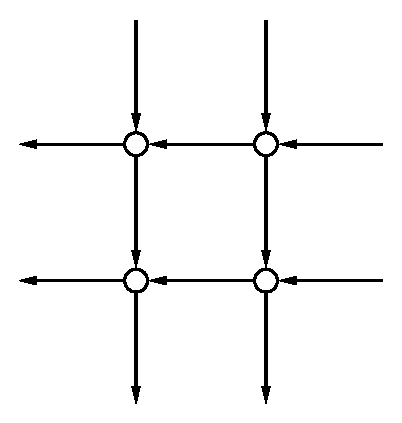
\includegraphics{figs/geometry}
      \end{picture}
      \setlength{\unitlength}{2279sp}
      \begingroup\makeatletter\ifx\SetFigFont\undefined
        \gdef\SetFigFont#1#2#3#4#5{
          \reset@font\fontsize{#1}{#2pt}
          \fontfamily{#3}\fontseries{#4}\fontshape{#5}
          \selectfont}
      \fi\endgroup
      \begin{picture}(5106,5376)(3748,-6574)
        \put(6301,-2851){\makebox(0,0)[b]{\smash{{\SetFigFont{9}{10.8}{\familydefault}{\mddefault}{\updefault}        $U_\mu(x+\hat\nu)$        }}}}
        \put(7291,-3931){\makebox(0,0)[lb]{\smash{{\SetFigFont{9}{10.8}{\familydefault}{\mddefault}{\updefault}        $U_\nu(x+\hat\mu)$        }}}}
        \put(4501,-4741){\makebox(0,0)[b]{\smash{{\SetFigFont{9}{10.8}{\familydefault}{\mddefault}{\updefault}        $U_\mu(x-\hat\mu)$        }}}}
        \put(6301,-4741){\makebox(0,0)[b]{\smash{{\SetFigFont{9}{10.8}{\familydefault}{\mddefault}{\updefault}        $U_\mu(x)$        }}}}
        \put(8101,-4741){\makebox(0,0)[b]{\smash{{\SetFigFont{9}{10.8}{\familydefault}{\mddefault}{\updefault}        $U_\mu(x+\hat\mu)$        }}}}
        \put(5491,-5821){\makebox(0,0)[lb]{\smash{{\SetFigFont{9}{10.8}{\familydefault}{\mddefault}{\updefault}        $U_\nu(x-\hat\nu)$        }}}}
        \put(7291,-5821){\makebox(0,0)[lb]{\smash{{\SetFigFont{9}{10.8}{\familydefault}{\mddefault}{\updefault}        $U_\nu(x+\hat\mu-\hat\nu)$        }}}}
        \put(5491,-3211){\makebox(0,0)[lb]{\smash{{\SetFigFont{9}{10.8}{\familydefault}{\mddefault}{\updefault}        $x+\hat\nu$        }}}}
        \put(7291,-3211){\makebox(0,0)[lb]{\smash{{\SetFigFont{9}{10.8}{\familydefault}{\mddefault}{\updefault}        $x+\hat\mu+\hat\nu$        }}}}
        \put(5491,-1951){\makebox(0,0)[lb]{\smash{{\SetFigFont{9}{10.8}{\familydefault}{\mddefault}{\updefault}        $U_\nu(x+\hat\mu)$        }}}}
        \put(7291,-1951){\makebox(0,0)[lb]{\smash{{\SetFigFont{9}{10.8}{\familydefault}{\mddefault}{\updefault}        $U_\nu(x+\hat\mu+\hat\nu)$        }}}}
        \put(5491,-3931){\makebox(0,0)[lb]{\smash{{\SetFigFont{9}{10.8}{\familydefault}{\mddefault}{\updefault}        $U_\nu(x)$        }}}}
        \put(7291,-5101){\makebox(0,0)[lb]{\smash{{\SetFigFont{9}{10.8}{\familydefault}{\mddefault}{\updefault}        $x+\hat\mu$        }}}}
        \put(5491,-5101){\makebox(0,0)[lb]{\smash{{\SetFigFont{9}{10.8}{\familydefault}{\mddefault}{\updefault}        $x$        }}}}
        \put(4456,-2851){\makebox(0,0)[b]{\smash{{\SetFigFont{9}{10.8}{\familydefault}{\mddefault}{\updefault}        $U_\mu(x-\hat\mu+\hat\nu)$        }}}}
        \put(8146,-2851){\makebox(0,0)[b]{\smash{{\SetFigFont{9}{10.8}{\familydefault}{\mddefault}{\updefault}        $U_\mu(x+\hat\mu+\hat\nu)$        }}}}
      \end{picture}
    }
    \caption{格上的命名约定。  }
    \label{geometry}
  \end{minipage}
  \hfill
  \begin{minipage}[t]{0.4\textwidth}
    \centering\scalebox{0.7}{\begin{picture}(0,0)
        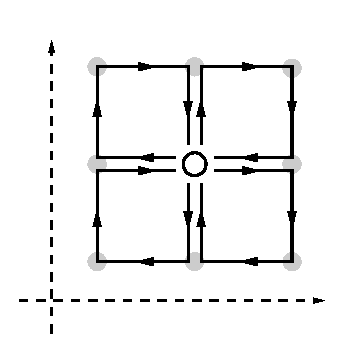
\includegraphics{figs/clover1}
      \end{picture}
      \setlength{\unitlength}{2279sp}
      \begingroup\makeatletter\ifx\SetFigFont\undefined
        \gdef\SetFigFont#1#2#3#4#5{
          \reset@font\fontsize{#1}{#2pt}
          \fontfamily{#3}\fontseries{#4}\fontshape{#5}
          \selectfont}
      \fi\endgroup
      \begin{picture}(4368,4392)(3388,-6664)
        \put(3781,-2491){\makebox(0,0)[lb]{\smash{{\SetFigFont{10}{12.0}{\familydefault}{\mddefault}{\updefault}        $\hat\nu$        }}}}
        \put(7741,-6271){\makebox(0,0)[lb]{\smash{{\SetFigFont{10}{12.0}{\familydefault}{\mddefault}{\updefault}        $\hat\mu$        }}}}
      \end{picture}
    }
    \caption{三叶草术语。  }
    \label{clover1}
  \end{minipage}
\end{figure}

连续理论的协变导数可以用多种方式离散化。在这里,我们将自己限制于广泛使用的 Wilson 离散化(参见~    \cite{Wilson:1975id}    ),并指出本文开发的多重网格求解器原则上适用于任何导致局部耦合的离散化。我们定义前向协变有限差分
$$
  \left(\Delta^\mu \psi_\sigma\right)(x) = \tfrac{1}{a}\left( {U_\mu(x) \psi_\sigma(x+\hat\mu) - \psi_\sigma(x)}\right)  \stackrel{\cdot}{=} (\partial_\mu + A_\mu) \psi_\sigma(x)
$$    和后向协变有限差分
$$
  \left(\Delta_\mu \psi_\sigma\right)(x) = \tfrac{1}{a} \left(\psi_\sigma(x) - U^H_{\mu}(x-\hat\mu) \psi_\sigma(x-\hat\mu)\right) \; .
$$    自    $( \Delta^\mu )^H = -\Delta_\mu$    以来,中心协变有限差分    $(\Delta^\mu + \Delta_\mu)/2$    是反厄米的。狄拉克算子    $\Dslash$    的最简单离散化由以下公式给出
$$ \textstyle
  D_N = \sum_{\mu=0}^3 \gamma_\mu \otimes \left(\Delta_\mu + \Delta^\mu\right)/2.
$$    这种简单的离散化会生成非物理的特征向量,这是使用中心有限差分离散化一阶导数时的标准现象,参见~    \cite{smith1985numerical}    ,也称为“物种倍增效应”或“红黑不稳定性”。    $D_N$    的每个特征值的特征空间都有维度    $16$    ,但只有一个一维子空间对应于连续算子的特征函数。为了避免这个问题,Wilson 引入了稳定项    $a\Delta_\mu \Delta^\mu$    ,即集中式二阶协变有限差分。因此,狄拉克算子的 Wilson 离散化由
\begin{equation}\label{WilsonDirac_eq}  \textstyle
  D_W = \frac{m_0}{a} I \;\; + \;\; \frac{1}{2} \sum_{\mu=0}^3 \Big( \gamma_\mu \otimes ( \Delta_\mu + \Delta^\mu ) - aI_4 \otimes \Delta_\mu \Delta^\mu \Big),
\end{equation}    给出,其中质量参数    $m_0$    设定夸克质量(有关更多详细信息,请参阅~    \cite{montvay1994quantum}    )。

$\gamma$    矩阵的交换关系    \eqref{commutativity_rel:eq}    意味着    $D_W$    具有非平凡对称性。定义    $\gamma_5 = \gamma_0\gamma_1\gamma_2\gamma_3$    后,我们得到    $\mu=0,1,2,3$    的    $\gamma_5 \gamma_\mu = - \gamma_\mu \gamma_5$    ,由于    $\gamma_\mu$    和    $\gamma_5$    是厄米算子,因此我们发现    $\gamma_5 \gamma_\mu$    是反厄米算子。因此算子    $(\gamma_5 \gamma_\mu) \otimes ( \Delta_\mu + \Delta^\mu)$    是厄米算子,是两个反厄米算子的乘积。为了描述 Wilson Dirac 算子的结果  {    \em       $\Gamma_5$   -对称性   }  ,我们定义    $\Gamma_5 = I_{n_{\mathcal{L}}} \otimes \gamma_5 \otimes I_3 $    并得到    $(\Gamma_5 D_W)^H = \Gamma_5 D_W$    。

为了降低    $a$    函数的离散化误差阶数,根据参数    $c_{sw}$    ,将 Sheik\-ho\-les\-la\-mi-Woh\-lert 或“三叶草”项(参见~    \cite{Sheikholeslami:1985ij}    和图    \ref{clover1}    )添加到格子 Wilson Dirac 算子
\begin{equation} \label{eq:lattice_WD}
  D = D_W \;\; - \;\; \frac{c_{sw}}{32a} \sum_{\mu,\nu=0}^3 ( \gamma_\mu \gamma_\nu ) \otimes ( Q_{\mu\nu} - Q_{\nu\mu} ),
\end{equation}    中,其中    $\left(Q_{\mu\nu}\psi_\sigma\right)(x) = Q_{\mu\nu}(x) \psi_\sigma(x)$    和
$$
  \begin{array}[h]{rcl}
    Q_{\mu\nu}(x) & = & U_{\mu}(x) \, U_{\nu}(x+\hat\mu) \, U_{\mu}(x+\hat\nu)^{H} \, U_{\nu}(x)^{H} +                                   \\
                  &   & U_{\nu}(x) \, U_{\mu}(x-\hat\mu+\hat\nu)^{H} \, U_{\nu}(x-\hat\mu)^{H} \, U_{ \mu}(x-\hat\mu) +                  \\
                  &   & U_{\mu}(x-\hat\mu)^{H} \, U_{\nu}(x-\hat\mu-\hat\nu)^{H} \, U_{ \mu}(x-\hat\mu-\hat\nu) \, U_{ \nu}(x-\hat\nu) + \\
                  &   & U_{\nu}(x-\hat\nu)^{H} \, U_{\mu}(x-\hat\nu) \, U_{ \nu}(x-\hat\nu+\hat\mu) \, U_{\mu}(x)^{H}.                   \\
  \end{array}
$$    三叶草项在格子    $\mathcal{L}$    上对角线。它从协变导数的协变有限差分离散化中消除了    $\mathcal{O}(a)$    离散化效应(对于适当调整的    $c_{\mathit{sw}}$    ;请参阅    \cite{Sheikholeslami:1985ij}    及其中的参考资料)。因此,得到的离散化狄拉克算子    $D$    具有阶数    $\mathcal{O}(a^2)$    的离散化效果。它再次是    $\Gamma_5$    对称的,即,我们有
\begin{equation} \label{eq:g5sym}
  (\Gamma_5 D)^H = \Gamma_5 D.
\end{equation}       $\Gamma_5$    对称性在    $D$    的频谱上引起对称性:

\begin{lemma} \label{lem:g5sym} Every right eigenvector         $\psi_\lambda$         to an eigenvalue         $\lambda$         of         $D$         corresponds to a left eigenvector         $\hat\psi_{\bar\lambda} = \Gamma_5 \psi_{\lambda}$
  to the eigenvalue         $\bar\lambda$         of         $D$         and vice versa. In particular, the spectrum of         $D$         is symmetric with respect to the real axis.
\end{lemma}

{    \em    证明。   }  由于    $D^H = \Gamma_5 D \Gamma_5$    我们有
\[
  D\psi_\lambda = \lambda\psi_\lambda \Leftrightarrow \psi_\lambda^H D^H = \bar{\lambda} \psi_\lambda^H \Leftrightarrow  (\Gamma_5 \psi_\lambda)^H D = \bar{\lambda} (\Gamma_5 \psi_\lambda)^H. \quad \quad \Box
\]

总结一下,   $D \in \mathbb{C}^{n\times n}$    是一个稀疏矩阵,它表示周期性 4D 晶格上的最近邻耦合。晶格有    $n_{\mathcal{L}} = N_tN_s^3$    个位点,每个位点有 12 个变量,因此    $n = 12n_{\mathcal{L}}$    。   $D$    具有对称性~    \eqref{eq:g5sym}    ,取决于质量参数    $m_0$    、Sheikholes\-la\-mi-Wohlert 常数    $c_{sw}$    和配置    $ \{  U_\mu(x) \, : \, x \in \mathcal{L} , \, \mu=0,1,2,3  \} $    。实际上    $m_0$    是负的,对于物理相关的质量参数,   $D$    的光谱包含在右半平面中,参见图~    \ref{figure:spectrum}    和图~    \ref{figure:spectrum_csw}    。

\begin{figure}
  \begin{minipage}[t]{0.48\textwidth}
    \centering\scalebox{0.65}{
      \begingroup
      \makeatletter
      \providecommand\color[2][]{
        \GenericError{(gnuplot) \space\space\space\@spaces}{
          Package color not loaded in conjunction with
          terminal option `colourtext'
        }{See the gnuplot documentation for explanation.
        }{Either use 'blacktext' in gnuplot or load the package
          color.sty in LaTeX.}
        \renewcommand\color[2][]{}
      }
      \providecommand\includegraphics[2][]{
        \GenericError{(gnuplot) \space\space\space\@spaces}{
          Package graphicx or graphics not loaded
        }{See the gnuplot documentation for explanation.
        }{The gnuplot epslatex terminal needs graphicx.sty or graphics.sty.}
        \renewcommand\includegraphics[2][]{}
      }
      \providecommand\rotatebox[2]{#2}
      \@ifundefined{ifGPcolor}{
        \newif\ifGPcolor
        \GPcolorfalse
      }{}
      \@ifundefined{ifGPblacktext}{
        \newif\ifGPblacktext
        \GPblacktexttrue
      }{}
      \let\gplgaddtomacro\g@addto@macro
      \gdef\gplbacktext{}
      \gdef\gplfronttext{}
      \makeatother
      \ifGPblacktext
        \def\colorrgb#1{}
        \def\colorgray#1{}
      \else
        \ifGPcolor
          \def\colorrgb#1{\color[rgb]{#1}}
          \def\colorgray#1{\color[gray]{#1}}
          \expandafter\def\csname LTw\endcsname{\color{white}}
          \expandafter\def\csname LTb\endcsname{\color{black}}
          \expandafter\def\csname LTa\endcsname{\color{black}}
          \expandafter\def\csname LT0\endcsname{\color[rgb]{1,0,0}}
          \expandafter\def\csname LT1\endcsname{\color[rgb]{0,1,0}}
          \expandafter\def\csname LT2\endcsname{\color[rgb]{0,0,1}}
          \expandafter\def\csname LT3\endcsname{\color[rgb]{1,0,1}}
          \expandafter\def\csname LT4\endcsname{\color[rgb]{0,1,1}}
          \expandafter\def\csname LT5\endcsname{\color[rgb]{1,1,0}}
          \expandafter\def\csname LT6\endcsname{\color[rgb]{0,0,0}}
          \expandafter\def\csname LT7\endcsname{\color[rgb]{1,0.3,0}}
          \expandafter\def\csname LT8\endcsname{\color[rgb]{0.5,0.5,0.5}}
        \else
          \def\colorrgb#1{\color{black}}
          \def\colorgray#1{\color[gray]{#1}}
          \expandafter\def\csname LTw\endcsname{\color{white}}
          \expandafter\def\csname LTb\endcsname{\color{black}}
          \expandafter\def\csname LTa\endcsname{\color{black}}
          \expandafter\def\csname LT0\endcsname{\color{black}}
          \expandafter\def\csname LT1\endcsname{\color{black}}
          \expandafter\def\csname LT2\endcsname{\color{black}}
          \expandafter\def\csname LT3\endcsname{\color{black}}
          \expandafter\def\csname LT4\endcsname{\color{black}}
          \expandafter\def\csname LT5\endcsname{\color{black}}
          \expandafter\def\csname LT6\endcsname{\color{black}}
          \expandafter\def\csname LT7\endcsname{\color{black}}
          \expandafter\def\csname LT8\endcsname{\color{black}}
        \fi
      \fi
      \setlength{\unitlength}{0.0500bp}
      \begin{picture}(4860.00,3402.00)
        \gplgaddtomacro\gplbacktext{
          \csname LTb\endcsname
          \put(860,640){\makebox(0,0)[r]{\strut{}        $-2$        }}
          \put(860,955){\makebox(0,0)[r]{\strut{}        $-1.5$        }}
          \put(860,1270){\makebox(0,0)[r]{\strut{}        $-1$        }}
          \put(860,1585){\makebox(0,0)[r]{\strut{}        $-0.5$        }}
          \put(860,1901){\makebox(0,0)[r]{\strut{}        $0$        }}
          \put(860,2216){\makebox(0,0)[r]{\strut{}        $0.5$        }}
          \put(860,2531){\makebox(0,0)[r]{\strut{}        $1$        }}
          \put(860,2846){\makebox(0,0)[r]{\strut{}        $1.5$        }}
          \put(860,3161){\makebox(0,0)[r]{\strut{}        $2$        }}
          \put(980,440){\makebox(0,0){\strut{}        $0$        }}
          \put(1420,440){\makebox(0,0){\strut{}        $1$        }}
          \put(1860,440){\makebox(0,0){\strut{}        $2$        }}
          \put(2300,440){\makebox(0,0){\strut{}        $3$        }}
          \put(2740,440){\makebox(0,0){\strut{}        $4$        }}
          \put(3179,440){\makebox(0,0){\strut{}        $5$        }}
          \put(3619,440){\makebox(0,0){\strut{}        $6$        }}
          \put(4059,440){\makebox(0,0){\strut{}        $7$        }}
          \put(4499,440){\makebox(0,0){\strut{}        $8$        }}
          \put(160,1900){\rotatebox{-270}{\makebox(0,0){\strut{}imaginary axis}}}
          \put(2739,140){\makebox(0,0){\strut{}real axis}}
        }
        \gplgaddtomacro\gplfronttext{
        }
        \gplbacktext
        \put(0,0){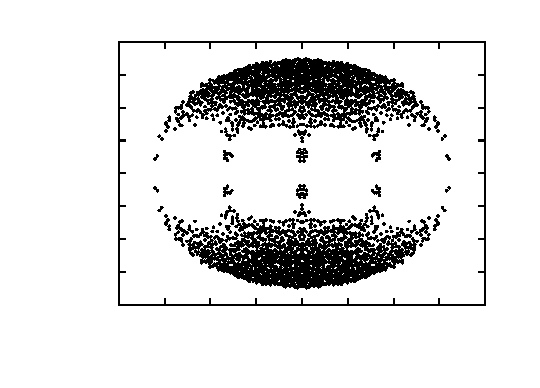
\includegraphics{./plots/plot_spectrum1}}
        \gplfronttext
      \end{picture}
      \endgroup
    }
    \caption{   $4^4$    威尔逊狄拉克算子的光谱;   $m_0 = 0$   、   $c_\mathit{sw} = 0$   。  }
    \label{figure:spectrum}
  \end{minipage}
  \hfill
  \begin{minipage}[t]{0.48\textwidth}
    \centering\scalebox{0.65}{
      \begingroup
      \makeatletter
      \providecommand\color[2][]{
        \GenericError{(gnuplot) \space\space\space\@spaces}{
          Package color not loaded in conjunction with
          terminal option `colourtext'
        }{See the gnuplot documentation for explanation.
        }{Either use 'blacktext' in gnuplot or load the package
          color.sty in LaTeX.}
        \renewcommand\color[2][]{}
      }
      \providecommand\includegraphics[2][]{
        \GenericError{(gnuplot) \space\space\space\@spaces}{
          Package graphicx or graphics not loaded
        }{See the gnuplot documentation for explanation.
        }{The gnuplot epslatex terminal needs graphicx.sty or graphics.sty.}
        \renewcommand\includegraphics[2][]{}
      }
      \providecommand\rotatebox[2]{#2}
      \@ifundefined{ifGPcolor}{
        \newif\ifGPcolor
        \GPcolorfalse
      }{}
      \@ifundefined{ifGPblacktext}{
        \newif\ifGPblacktext
        \GPblacktexttrue
      }{}
      \let\gplgaddtomacro\g@addto@macro
      \gdef\gplbacktext{}
      \gdef\gplfronttext{}
      \makeatother
      \ifGPblacktext
        \def\colorrgb#1{}
        \def\colorgray#1{}
      \else
        \ifGPcolor
          \def\colorrgb#1{\color[rgb]{#1}}
          \def\colorgray#1{\color[gray]{#1}}
          \expandafter\def\csname LTw\endcsname{\color{white}}
          \expandafter\def\csname LTb\endcsname{\color{black}}
          \expandafter\def\csname LTa\endcsname{\color{black}}
          \expandafter\def\csname LT0\endcsname{\color[rgb]{1,0,0}}
          \expandafter\def\csname LT1\endcsname{\color[rgb]{0,1,0}}
          \expandafter\def\csname LT2\endcsname{\color[rgb]{0,0,1}}
          \expandafter\def\csname LT3\endcsname{\color[rgb]{1,0,1}}
          \expandafter\def\csname LT4\endcsname{\color[rgb]{0,1,1}}
          \expandafter\def\csname LT5\endcsname{\color[rgb]{1,1,0}}
          \expandafter\def\csname LT6\endcsname{\color[rgb]{0,0,0}}
          \expandafter\def\csname LT7\endcsname{\color[rgb]{1,0.3,0}}
          \expandafter\def\csname LT8\endcsname{\color[rgb]{0.5,0.5,0.5}}
        \else
          \def\colorrgb#1{\color{black}}
          \def\colorgray#1{\color[gray]{#1}}
          \expandafter\def\csname LTw\endcsname{\color{white}}
          \expandafter\def\csname LTb\endcsname{\color{black}}
          \expandafter\def\csname LTa\endcsname{\color{black}}
          \expandafter\def\csname LT0\endcsname{\color{black}}
          \expandafter\def\csname LT1\endcsname{\color{black}}
          \expandafter\def\csname LT2\endcsname{\color{black}}
          \expandafter\def\csname LT3\endcsname{\color{black}}
          \expandafter\def\csname LT4\endcsname{\color{black}}
          \expandafter\def\csname LT5\endcsname{\color{black}}
          \expandafter\def\csname LT6\endcsname{\color{black}}
          \expandafter\def\csname LT7\endcsname{\color{black}}
          \expandafter\def\csname LT8\endcsname{\color{black}}
        \fi
      \fi
      \setlength{\unitlength}{0.0500bp}
      \begin{picture}(4860.00,3402.00)
        \gplgaddtomacro\gplbacktext{
          \csname LTb\endcsname
          \put(860,640){\makebox(0,0)[r]{\strut{}        $-2$        }}
          \put(860,955){\makebox(0,0)[r]{\strut{}        $-1.5$        }}
          \put(860,1270){\makebox(0,0)[r]{\strut{}        $-1$        }}
          \put(860,1585){\makebox(0,0)[r]{\strut{}        $-0.5$        }}
          \put(860,1901){\makebox(0,0)[r]{\strut{}        $0$        }}
          \put(860,2216){\makebox(0,0)[r]{\strut{}        $0.5$        }}
          \put(860,2531){\makebox(0,0)[r]{\strut{}        $1$        }}
          \put(860,2846){\makebox(0,0)[r]{\strut{}        $1.5$        }}
          \put(860,3161){\makebox(0,0)[r]{\strut{}        $2$        }}
          \put(980,440){\makebox(0,0){\strut{}        $0$        }}
          \put(1420,440){\makebox(0,0){\strut{}        $1$        }}
          \put(1860,440){\makebox(0,0){\strut{}        $2$        }}
          \put(2300,440){\makebox(0,0){\strut{}        $3$        }}
          \put(2740,440){\makebox(0,0){\strut{}        $4$        }}
          \put(3179,440){\makebox(0,0){\strut{}        $5$        }}
          \put(3619,440){\makebox(0,0){\strut{}        $6$        }}
          \put(4059,440){\makebox(0,0){\strut{}        $7$        }}
          \put(4499,440){\makebox(0,0){\strut{}        $8$        }}
          \put(160,1900){\rotatebox{-270}{\makebox(0,0){\strut{}imaginary axis}}}
          \put(2739,140){\makebox(0,0){\strut{}real axis}}
        }
        \gplgaddtomacro\gplfronttext{
        }
        \gplbacktext
        \put(0,0){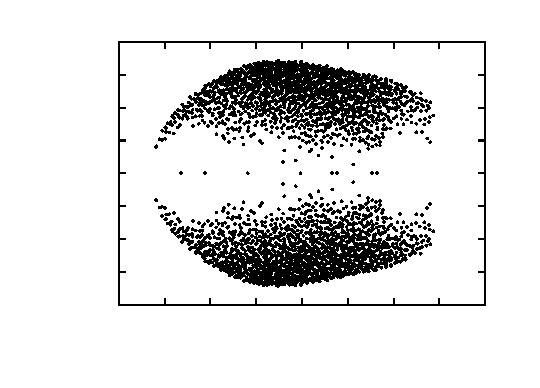
\includegraphics{./plots/plot_spectrum1csw}}
        \gplfronttext
      \end{picture}
      \endgroup
    }
    \caption{   $4^4$   “Clover 改进”算子的频谱;   $m_0 = 0$   、   $c_\mathit{sw} = 1$   。  }
    \label{figure:spectrum_csw}
  \end{minipage}
\end{figure}

连续狄拉克算子是正态的,而威尔逊狄拉克算子不是,但当离散化效应变小时,它会趋近于正态。因此,对于较小的晶格间距、较大的晶格尺寸和物理相关的质量参数,我们可以预期    $\mathcal{F}(D) =  \{  \psi^HD\psi : \psi^H\psi = 1 \} $    和    $D$    的整个值场都在右半平面中。

为了以矩阵形式明确地表达    $D$   ,我们将    $\gamma$    矩阵的表示固定为
\begin{equation*}\label{eq:chiralgamma}
  \gamma_{0} = \small{
    \begin{pmatrix}
      \phantom{i}                            & \phantom{i}                            & \phantom{i} & i           \\
                                             &                                        & i           & \phantom{i} \\
                                             & \makebox[0cm][c]{        $-i$        } &             &             \\
      \makebox[0cm][c]{        $-i$        } &                                        &             &
    \end{pmatrix}},
  \gamma_{1} = \small{ \left( \;
    \begin{matrix}
      \phantom{1}                            & \phantom{1} & \phantom{1} & \makebox[0cm][c]{        $-1$        } \\
                                             &             & 1           & \phantom{1}                            \\
                                             & 1           &             &                                        \\
      \makebox[0cm][c]{        $-1$        } &             &             &
    \end{matrix}
    \; \right)},
  \gamma_{2} = \small{ \left(
    \begin{matrix}
      \phantom{i}                            & \phantom{i} & i           & \phantom{i}                            \\
                                             &             & \phantom{i} & \makebox[0cm][c]{        $-i$        } \\
      \makebox[0cm][c]{        $-i$        } &             &             &                                        \\
                                             & i           &             &
    \end{matrix}
    \; \right)},
  \gamma_{3} = \small{
    \begin{pmatrix}
      \phantom{1} & \phantom{1} & 1          & \phantom{1} \\
                  &             & \phantom{} & 1           \\
      1           &             &            &             \\
                  & 1           &            &
    \end{pmatrix}
  },
\end{equation*}    ,结果为
\[
  \gamma_5 = \diag(1,1,-1-1).
\]    因此,   $\gamma_5$    在自旋 0 和 1 上充当恒等式,在自旋 2 和 3 上充当负恒等式。然后通过以下方式给出    $D$
\begin{eqnarray*}
  (D\psi)(x) &=& \frac{1}{a} \Big( (m_0+4) I_{12} - \frac{c_{sw}}{32} \sum_{\mu,\nu=0}^3 ( \gamma_\mu \gamma_\nu ) \otimes \big( Q_{\mu\nu}(x) - Q_{\nu\mu}(x) \big) \Big) \psi(x)  \\
  & &  \mbox{} - \frac{1}{2a}\sum_{\mu=0}^3 \left( (I_4-\gamma_\mu)\otimes U_\mu(x)\right) \psi(x+\hat{\mu})  \\
  & & \mbox{} - \frac{1}{2a}\sum_{\mu=0}^3 \left( (I_4+\gamma_\mu)\otimes U_\mu^H(x-\hat{\mu})\right) \psi(x-\hat{\mu}) .
\end{eqnarray*}
\subsection{格点 QCD 中的域分解  }       \label{dd_in_lattice_qcd}    为了便于表示,我们从现在开始删除晶格间距    $a$    ,因此晶格    $\mathcal{L}$    给出为
\[
  \mathcal{L} =  \{  x = (x_0,x_1,x_2,x_3), 1 \leq x_0 \leq N_t, \, 1 \leq x_1,x_2,x_3 \leq N_s  \} .
\]

我们还保留术语  {    \em    块分解   } ,用于将    $\mathcal{L}$    张量类型分解为格块。精确定义如下。

\begin{definition}
  Assume that         $ \{  \mathcal{T}^0_{1},\ldots, \mathcal{T}^0_{\ell_0} \} $         is a partitioning of         $ \{ 1,\ldots,N_t \} $         into         $\ell_0$         blocks of consecutive time points,
  \[
    \mathcal{T}^0_{j} =  \{  t_{j-1}+1,\ldots,t_{j} \} , \quad j=1,\ldots,\ell_0, \, 0=t_0 < t_1 \ldots < t_{\ell_0} = N_t,
  \]
  and similarly for the spatial dimensions with partitionings         $ \{  \mathcal{T}^\mu_{1},\ldots, \mathcal{T}^\mu_{\ell_\mu} \} , \, \mu=1,2,3$        .

  A {\em block decomposition} of         $\mathcal{L}$         is a partitioning of         $\mathcal{L}$         into         $\ell= \ell_0\ell_1\ell_2\ell_3$         lattice-blocks         $\mathcal{L}_i$        , where each lattice-block is of the form
  \[
    \mathcal{L}_i = \mathcal{T}^0_{j_0(i)} \times \mathcal{T}^1_{j_1(i)} \times \mathcal{T}^2_{j_2(i)} \times \mathcal{T}^3_{j_3(i)}.
  \]
  Accordingly we define a block decomposition of all         $12n_\mathcal{L}$         variables in         $\mathcal{V} = \mathcal{L}\times\mathcal{C}\times\mathcal{S}$         into         $\ell$         blocks         $\mathcal{V}_i$         by grouping all spin and color components from the lattice-block         $\mathcal{L}_i$        ,
  \begin{equation} \label{eq:variable_blocks}
    \mathcal{V}_i = \mathcal{L}_i\times\mathcal{C}\times\mathcal{S}.
  \end{equation}
\end{definition}

由于格点 QCD 计算中出现的系统往往有数亿个未知数,因此需要使用并行计算机。出于这个原因,并且由于通常已经使用简单的域分解来并行化 Krylov 子空间方法所需的矩阵向量积    $Dz$   ,因此自然也会使用域分解方法作为预处理器。

这里选择的方法是乘法施瓦茨方法    \cite{Schwarz1870, BFSmith_PEBjorstad_WDGropp_1996a}    的彩色版本。由于离散化的狄拉克算子只有最近邻耦合,因此只需要两种颜色。对于根据    \eqref{eq:variable_blocks}    对格和变量块    $\mathcal{V}_i$    进行块分解,让相应的平凡嵌入、块系统和块求解器表示为
\[
  \mathcal{I}_{\mathcal{V}_i} :  \mathcal{V}_i \rightarrow \mathcal{V}, \quad D_i = \mathcal{I}_{\mathcal{V}_i}^T D \mathcal{I}_{\mathcal{V}_i} \quad \text{and} \quad B_i = \mathcal{I}_{\mathcal{V}_i} D_i^{-1} \mathcal{I}_{\mathcal{V}_i}^T.
\]    对于红黑乘法施瓦茨,格块分为两组(红色和黑色),使得    $D$    中的任何方程都不会耦合来自相同颜色的不同块的变量。给定残差    $r=b-Dx$    ,局部系统    \begin{equation} \label{eq:localsystem}
  D_i e_i =  \mathcal{I}_{\mathcal{V}_i}^Tr,
\end{equation}    的解    $e_i$    产生迭代    $x$    的修正。更准确地说,使用简写    $B_{color} = \sum_{i \in \text{\it color \  }} B_{i}$    和
\[
  K = B_{\text{\it black \  }}(I - D\, B_{\text{\it red \  }}) + B_{\text{\it red \  }}
\]    ,我们可以将红黑乘法 Schwarz 的一次迭代 (    $\nu = 1$    ) 总结为 (参见~    \cite{BFSmith_PEBjorstad_WDGropp_1996a}    )
\begin{equation} \label{SAP_1step:eq}
  z \leftarrow (I-KD)z + Kb.
\end{equation}    由于解    $z^* = D^{-1}b$    满足    $z^* = (I-KD)z^* + Kb$    ,因此误差的更新为
$e \leftarrow (I-KD)e$    ,其中    $I-KD$    为误差传播运算符,
\begin{equation*}
  \ESAP = I - KD = (I-B_{\text{\it black \  }}D)(I-B_{\text{\it red \  }}D) \, .
\end{equation*}

红黑施瓦茨方法在~    \cite{Luescher2003}    中被引入到格点 QCD 中,并且从那时起就被用作多个格点 QCD 实现中的预处理器(参见~    \cite{Aoki:2008sm,Nobile2012,Luescher2007}    )。在这种情况下,红黑施瓦茨也称为施瓦茨交替程序 (SAP)。接下来,将 SAP 的    $\nu$    次迭代应用于向量    $b$    ,初始猜测    $z=0$    用线性算子    \begin{equation*}
  \MSAP{\nu} b = \sum_{k=0}^{\nu-1} (I-KD)^k \, K \, b \,.
\end{equation*}    表示。此表示随后是    \eqref{SAP_1step:eq}    的重复应用。请注意,   $ \ESAP = I - \MSAPone D $    与    $ \MSAPone = \MSAP{1} $    。

\begin{figure}[ht]
  \begin{minipage}[t]{0.45\textwidth}
    \centering \scalebox{0.9}{\begin{picture}(0,0)
        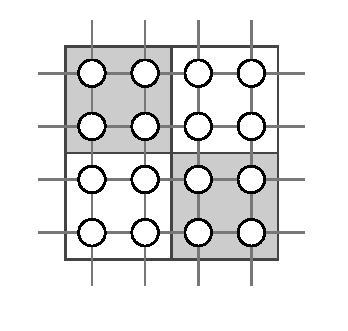
\includegraphics{figs/redblack_small}
      \end{picture}
      \setlength{\unitlength}{1865sp}
      \begingroup\makeatletter\ifx\SetFigFont\undefined
        \gdef\SetFigFont#1#2#3#4#5{
          \reset@font\fontsize{#1}{#2pt}
          \fontfamily{#3}\fontseries{#4}\fontshape{#5}
          \selectfont}
      \fi\endgroup
      \begin{picture}(5295,5016)(526,-4819)
        \put(541,-3031){\makebox(0,0)[b]{\smash{{\SetFigFont{10}{12.0}{\familydefault}{\mddefault}{\updefault}        $\mathcal{L}_3$        }}}}
        \put(541,-1231){\makebox(0,0)[b]{\smash{{\SetFigFont{10}{12.0}{\familydefault}{\mddefault}{\updefault}        $\mathcal{L}_1$        }}}}
        \put(5806,-1231){\makebox(0,0)[b]{\smash{{\SetFigFont{10}{12.0}{\familydefault}{\mddefault}{\updefault}        $\mathcal{L}_2$        }}}}
        \put(5806,-3076){\makebox(0,0)[b]{\smash{{\SetFigFont{10}{12.0}{\familydefault}{\mddefault}{\updefault}        $\mathcal{L}_4$        }}}}
        \put(3106,-4696){\makebox(0,0)[b]{\smash{{\SetFigFont{10}{12.0}{\familydefault}{\mddefault}{\updefault}        $\mathcal{L}$        }}}}
      \end{picture}
    }
    \caption{块分解格(简化为    $2$    D),具有    $2$    颜色  }
    \label{redblack_small}
  \end{minipage}
  \hfill
  \begin{minipage}[t]{0.5\textwidth}
    \centering \scalebox{0.74}{
      \begingroup
      \makeatletter
      \providecommand\color[2][]{
        \GenericError{(gnuplot) \space\space\space\@spaces}{
          Package color not loaded in conjunction with
          terminal option `colourtext'
        }{See the gnuplot documentation for explanation.
        }{Either use 'blacktext' in gnuplot or load the package
          color.sty in LaTeX.}
        \renewcommand\color[2][]{}
      }
      \providecommand\includegraphics[2][]{
        \GenericError{(gnuplot) \space\space\space\@spaces}{
          Package graphicx or graphics not loaded
        }{See the gnuplot documentation for explanation.
        }{The gnuplot epslatex terminal needs graphicx.sty or graphics.sty.}
        \renewcommand\includegraphics[2][]{}
      }
      \providecommand\rotatebox[2]{#2}
      \@ifundefined{ifGPcolor}{
        \newif\ifGPcolor
        \GPcolorfalse
      }{}
      \@ifundefined{ifGPblacktext}{
        \newif\ifGPblacktext
        \GPblacktexttrue
      }{}
      \let\gplgaddtomacro\g@addto@macro
      \gdef\gplbacktext{}
      \gdef\gplfronttext{}
      \makeatother
      \ifGPblacktext
        \def\colorrgb#1{}
        \def\colorgray#1{}
      \else
        \ifGPcolor
          \def\colorrgb#1{\color[rgb]{#1}}
          \def\colorgray#1{\color[gray]{#1}}
          \expandafter\def\csname LTw\endcsname{\color{white}}
          \expandafter\def\csname LTb\endcsname{\color{black}}
          \expandafter\def\csname LTa\endcsname{\color{black}}
          \expandafter\def\csname LT0\endcsname{\color[rgb]{1,0,0}}
          \expandafter\def\csname LT1\endcsname{\color[rgb]{0,1,0}}
          \expandafter\def\csname LT2\endcsname{\color[rgb]{0,0,1}}
          \expandafter\def\csname LT3\endcsname{\color[rgb]{1,0,1}}
          \expandafter\def\csname LT4\endcsname{\color[rgb]{0,1,1}}
          \expandafter\def\csname LT5\endcsname{\color[rgb]{1,1,0}}
          \expandafter\def\csname LT6\endcsname{\color[rgb]{0,0,0}}
          \expandafter\def\csname LT7\endcsname{\color[rgb]{1,0.3,0}}
          \expandafter\def\csname LT8\endcsname{\color[rgb]{0.5,0.5,0.5}}
        \else
          \def\colorrgb#1{\color{black}}
          \def\colorgray#1{\color[gray]{#1}}
          \expandafter\def\csname LTw\endcsname{\color{white}}
          \expandafter\def\csname LTb\endcsname{\color{black}}
          \expandafter\def\csname LTa\endcsname{\color{black}}
          \expandafter\def\csname LT0\endcsname{\color{black}}
          \expandafter\def\csname LT1\endcsname{\color{black}}
          \expandafter\def\csname LT2\endcsname{\color{black}}
          \expandafter\def\csname LT3\endcsname{\color{black}}
          \expandafter\def\csname LT4\endcsname{\color{black}}
          \expandafter\def\csname LT5\endcsname{\color{black}}
          \expandafter\def\csname LT6\endcsname{\color{black}}
          \expandafter\def\csname LT7\endcsname{\color{black}}
          \expandafter\def\csname LT8\endcsname{\color{black}}
        \fi
      \fi
      \setlength{\unitlength}{0.0500bp}
      \begin{picture}(4860.00,3402.00)
        \gplgaddtomacro\gplbacktext{
          \csname LTb\endcsname
          \put(740,640){\makebox(0,0)[r]{\strut{}        $0$        }}
          \put(740,1098){\makebox(0,0)[r]{\strut{}        $0.2$        }}
          \put(740,1557){\makebox(0,0)[r]{\strut{}        $0.4$        }}
          \put(740,2015){\makebox(0,0)[r]{\strut{}        $0.6$        }}
          \put(740,2473){\makebox(0,0)[r]{\strut{}        $0.8$        }}
          \put(740,2932){\makebox(0,0)[r]{\strut{}        $1$        }}
          \put(860,440){\makebox(0,0){\strut{}        $0$        }}
          \put(1447,440){\makebox(0,0){\strut{}        $500$        }}
          \put(2034,440){\makebox(0,0){\strut{}        $1000$        }}
          \put(2621,440){\makebox(0,0){\strut{}        $1500$        }}
          \put(3208,440){\makebox(0,0){\strut{}        $2000$        }}
          \put(3795,440){\makebox(0,0){\strut{}        $2500$        }}
          \put(4382,440){\makebox(0,0){\strut{}        $3000$        }}
          \put(160,1900){\rotatebox{-270}{\makebox(0,0){\strut{}        $||E_\mathit{SAP} \, v_i||/||v_i||$        }}}
          \put(2679,140){\makebox(0,0){\strut{}number of eigenvalue}}
        }
        \gplgaddtomacro\gplfronttext{
        }
        \gplbacktext
        \put(0,0){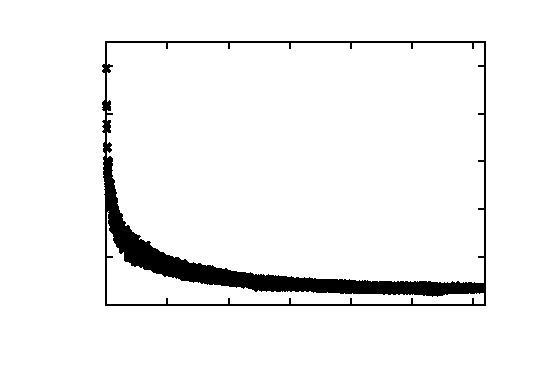
\includegraphics{./plots/plot_smoother_on_spectrum}}
        \gplfronttext
      \end{picture}
      \endgroup
    }
    \caption{在块大小为    $2^4$    的    $4^4$    格子上减少误差分量  }
    \label{errSAP}
  \end{minipage}
\end{figure}

通常,计算    $B_ir$    时所需的局部系统    \eqref{eq:localsystem}    的解是通过 Krylov 子空间方法(例如 GMRES)的几次迭代来近似的。当结合这种近似求解器时,SAP 方法就变成了非平稳迭代过程。因此,如果 SAP 用作预处理器(参见~    \cite{Nobile2012, Luescher2003, Saad:2003:IMS:829576}    ),则必须使用灵活的 Krylov 子空间方法,如 FGMRES 或 GCR。

事实证明,SAP 作为预处理器无法弥补 Krylov 子空间方法在系统大小、夸克质量和物理体积方面的不利缩放行为。分析这种行为时,人们会发现 SAP 可以很好地减少属于大部分频谱的误差分量,但一小部分几乎不受 SAP 的影响。我们在图    \ref{errSAP}    中说明了这一点,其中横轴表示    $D$    的特征向量    $v$   ,按相应特征值的绝对值升序排列;纵轴给出比率    $\|\ESAP v\|/\|v\|$    。对于较大的特征值,该比率较小,而对于较小的特征值,该比率会变得明显较大。这种行为是代数多重网格方法中平滑器的典型行为,这促使我们在这种情况下使用 SAP。
\section{代数多重网格方法  }       \label{section:AMG}    任何多重网格方法都由两个组件组成,一个平滑器和一个粗网格校正    \cite{Brezina2005,hackbusch2003multi,RugeStueben87,UTrottenberg_etal_2001}    。通常,平滑器可以选择简单的迭代方法。这可以是松弛方案,如 Jacobi 或 Gauss-Seidel 或它们的块变体以及 Krylov 子空间方法。鉴于上一节中介绍的 SAP 的属性,我们选择 SAP 作为 QCD 环境中的平滑方案。

我们将项  {    \em    靠近内核   }  保留用于由属于    $D$    的小(模数)特征值的特征向量所跨越的空间。由于 SAP 无法充分去除属于近核的误差分量(参见图    \ref{errSAP}   ),多重网格方法在具有    $n_c$    变量的较小子空间中分别处理这些持久误差分量。因此,该子空间应近似于近核。典型的代数多重网格设置如下:我们必须找到一个算子    $D_c$   ,它在该子空间上类似于    $D$   ,不仅因为它以与    $D$    类似的方式作用于近核,而且在连接结构和稀疏性方面也如此。后者允许使用相同方法递归地对    $D_c$    进行操作,从而从二网格变为真正的多重网格。我们还需要一个线性映射    $R: \mathbb{C}^{n} \rightarrow \mathbb{C}^{n_c}$    来将信息从原始空间限制到子空间,以及一个线性映射    $P: \mathbb{C}^{n_c} \rightarrow \mathbb{C}^{n}$    将信息传输回原始空间。然后通过将残差    $r= b-Dz$    限制到子空间,获得原始空间上当前迭代    $z$    的粗网格校正,在那里求解
\begin{equation} \label{coarse_eq}
  D_c e_c = Rr
\end{equation}    并将粗误差    $e_c$    传输回原始空间作为    $z$    的校正,从而得到子空间校正
\begin{equation} \label{coarse_grid_correction}
  z \leftarrow z + P D_c^{-1} R r, \, \quad r=b-Dz
\end{equation}    和相应的误差传播器
$$
  I - P D_c^{-1} R D.
$$

通常,粗网格系统是通过关于    $P$    和    $R$    的 Petrov-Galerkin 投影获得的,即
\[
  D_c = RDP.
\]    粗网格校正    $I-P(RDP)^{-1}RD$    是沿    $\range(P)$    投影到    $\range(RD)^\perp$    上的投影。如果    $\range(P)$    近似包含近核,而    $\range(RD)^\perp$    近似包含剩余的互补特征向量(然后由平滑器有效地减少),则粗网格校正的作用与平滑器的作用互补。如果    $\range(R)$    近似包含与小特征值相对应的  {    \em    剩余   }  特征向量,则满足后一个条件。通过查看精确的特征向量可以看出:由于左特征向量和右特征向量相互正交,如果    $\range(R)= \range(RD)$    由    $D$    的左特征向量跨越,则    $\range(R)^\perp$    由    $D$    的互补右特征向量跨越。

一旦找到    $D_c$   ,一个基本的两级算法就由交替应用平滑器和粗网格校正组成。通过为    \eqref{coarse_eq}    的解制定这种两级算法,可以将此过程递归扩展为真正的多重网格,直到我们获得一个足够小的算子来直接解决    \eqref{coarse_eq}   。

为了在计算上有利,求解    \eqref{coarse_eq}    必须比求解原始方程    $Dz = b$    便宜得多。为此,   $D_c$    必须非常小或稀疏。随着 SAP 平滑器未充分减少的特征向量数量随着    $n$    的增长而增长,参见~    \cite{Banks:1979yr}    ,我们不应该以修复    $n_c$    为目标(如在缩减方法中),而应该以找到稀疏矩阵    $R$    和    $P$    为目标,它们的范围分别很好地近似于    $D$    的左和右近核。
\subsection{基于聚合的电网间传输运营商  }       \label{sec:aggAMG}    考虑使用格块    $\mathcal{L}_i$    对格    $\mathcal{L}$    进行块分解。在    \cite{Luescher2007}    中观察到,属于    $D$    的小特征值的特征向量往往(近似地)在大量格块    $\mathcal{L}_i$    上重合,这种现象被称为“局部相干性”。局部相干性特别意味着我们可以通过将许多特征向量分解为属于每个格块的部分,用少数几个小特征值来表示它们。我们参考~    \cite{Luescher2007}    来详细定性分析这一观察结果。局部相干性是基于聚合的网格间传输算子背后的哲学,该算子在    \cite{DBraess_1995, Brezina2005}    中以一般设置引入,并在
\cite{MGClark2010_1,MGClark2007,MGClark2010_2}    中应用于 QCD 问题。

\begin{definition} An {\em aggregation}         $ \{ \mathcal{A}_1,\ldots,\mathcal{A}_s \} $         is a partitioning of the set         $\mathcal{V} = \mathcal{L}\times\mathcal{C}\times\mathcal{S}$         of all variables. It is termed a {\em lattice-block based} aggregation if each         $\mathcal{A}_i$         is of the form
  \[
    \mathcal{A}_i = \mathcal{L}_{j(i)} \times \mathcal{W}_{i},
  \]
  where         $\mathcal{L}_j$         are the lattice-blocks of a block decomposition of         $\mathcal{L}$         and         $\mathcal{W}_i \subseteq \mathcal{C} \times \mathcal{S}$        .
\end{definition}

格 Wilson Dirac 算子    \eqref{eq:lattice_WD}    的聚合通常将实现为基于格块的聚合。但请注意,一方面是 SAP 平滑器,另一方面是插值和限制,不必基于    $\mathcal{L}$    的  {    \em    普通   }  块分解。

从一组表示近核的  {    \em    测试向量   }     $ \{  v_1,\ldots, v_N  \} $    和一组聚合体    $  \{  \mathcal{A}_1,\ldots, \mathcal{A}_s  \}  $    开始,通过分解聚合体上的测试向量获得插值    $P$

\begin{equation}\label{eq:aggInterpolation}
  (v_1 \mid \ldots \mid v_N) =
  \left( \begin{array}{|c|}
      \hline
      \cline{1-1}
      \multicolumn{1}{|c|}{} \\
      \multicolumn{1}{|c|}{} \\
      \multicolumn{1}{|c|}{} \\
      \multicolumn{1}{|c|}{} \\
      \multicolumn{1}{|c|}{} \\
      \multicolumn{1}{|c|}{} \\
      \multicolumn{1}{|c|}{} \\
      \hline
    \end{array} \right)
  \longrightarrow
  P = \left( \begin{array}{c c c c c c c c}
      \cline{1-1}
      \multicolumn{1}{|c|}{} &                        &        &                        \\
      \multicolumn{1}{|c|}{} &                        &        &                        \\
      \cline{1-2}
                             & \multicolumn{1}{|c|}{} &        &                        \\
                             & \multicolumn{1}{|c|}{} &        &                        \\
      \cline{2-2}
                             &                        & \ddots &                        \\
      \cline{4-4}
                             &                        &        & \multicolumn{1}{|c|}{} \\
                             &                        &        & \multicolumn{1}{|c|}{} \\
      \cline{4-4}
    \end{array} \right)
  \begin{array}{c}
    \multirow{2}{*}{        $\mathcal{A}_1$        } \\
    \\
    \multirow{2}{*}{        $\mathcal{A}_2$        } \\
    \\
    \vdots                                           \\
    \multirow{2}{*}{        $\mathcal{A}_s$        } \\
    \\
  \end{array}.
\end{equation}    形式上,每个聚合体    $\mathcal{A}_i$    在粗系统上诱导    $N$    变量    $(i-1)N+1,\ldots, iN$   ,我们定义

\begin{equation} \label{eq:aggInterpolation2}
  Pe_{(i-1)N+j} = \mathcal{I}^T_{\mathcal{A}_i}v_j, \quad i=1,\ldots,s, \, j=1,\ldots,N.
\end{equation}    其中,   $\mathcal{I}_{\mathcal{A}_i}$    表示聚合体    $\mathcal{A}_i$    的平凡限制运算符,即,   $\mathcal{I}^T_{\mathcal{A}_i}v_j$    保持    $\mathcal{A}_{i}$    中    $v_j$    的分量不变,同时将所有其他分量归零,   $e_{(i-1)N+j}$    表示    $(i-1)N+j$    第单位向量。为了稳定性,测试向量在局部进行了正交归一化,即,对于每个    $i$    ,我们将    \eqref{eq:aggInterpolation2}    中的    $\mathcal{I}_{\mathcal{A}_i}^Tv_j$    替换为    $\mbox{span}(\mathcal{I}^T_{\mathcal{A}_i}v_1,\ldots,\mathcal{I}^T_{\mathcal{A}_i}v_N)$    正交基的第    $j$    个基向量。这不会改变    $P$    的范围,也不会改变粗网格校正算子    $I-P(RDP)^{-1}RD$    ,并确保    $P^HP = I$    。

通过使用一组测试向量    $ \{  \hat{v}_1,\ldots, \hat{v}_N  \} $    和相同的聚合来构建    $R^H$    ,可以以类似的方式获得限制    $R$    。图    \ref{aggregation}    从格点(再次简化为二维)说明了基于格块的聚合,其中在每个聚合    $\mathcal{A}$    中,我们将    $\mathcal{W}_i$    视为整个集合    $\mathcal{C} \times \mathcal{S}$    。然后,可以将聚合视为形成一个新的粗格,并且    $D_c = RDP$    的稀疏性和连接结构类似于    $D$    的稀疏性和连接结构,即我们再次具有最近邻耦合。粗网格的每个格点(即每个聚合)都包含    $N$    变量。

\begin{figure}[ht]
  \centering \scalebox{0.7}{\begin{picture}(0,0)
      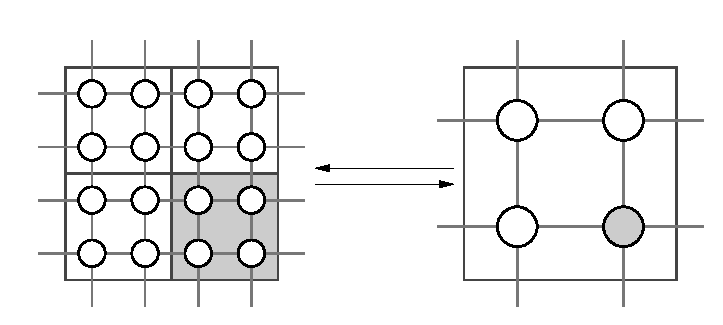
\includegraphics{figs/aggregation2}
    \end{picture}
    \setlength{\unitlength}{1865sp}
    \begingroup\makeatletter\ifx\SetFigFont\undefined
      \gdef\SetFigFont#1#2#3#4#5{
        \reset@font\fontsize{#1}{#2pt}
        \fontfamily{#3}\fontseries{#4}\fontshape{#5}
        \selectfont}
    \fi\endgroup
    \begin{picture}(11658,4935)(526,-4369)
      \put(541,-3031){\makebox(0,0)[b]{\smash{{\SetFigFont{10}{12.0}{\familydefault}{\mddefault}{\updefault}        $\mathcal{A}_3$        }}}}
      \put(541,-1231){\makebox(0,0)[b]{\smash{{\SetFigFont{10}{12.0}{\familydefault}{\mddefault}{\updefault}        $\mathcal{A}_1$        }}}}
      \put(5806,-1231){\makebox(0,0)[b]{\smash{{\SetFigFont{10}{12.0}{\familydefault}{\mddefault}{\updefault}        $\mathcal{A}_2$        }}}}
      \put(5806,-3076){\makebox(0,0)[b]{\smash{{\SetFigFont{10}{12.0}{\familydefault}{\mddefault}{\updefault}        $\mathcal{A}_4$        }}}}
      \put(7246,-2671){\makebox(0,0)[b]{\smash{{\SetFigFont{10}{12.0}{\familydefault}{\mddefault}{\updefault}        $R$        }}}}
      \put(7201,-1861){\makebox(0,0)[b]{\smash{{\SetFigFont{10}{12.0}{\familydefault}{\mddefault}{\updefault}        $P$        }}}}
      \put(3151,299){\makebox(0,0)[b]{\smash{{\SetFigFont{10}{12.0}{\familydefault}{\mddefault}{\updefault}        $D$        }}}}
      \put(9901,299){\makebox(0,0)[b]{\smash{{\SetFigFont{10}{12.0}{\familydefault}{\mddefault}{\updefault}        $D_c$        }}}}
    \end{picture}
  }
  \caption{基于聚合的插值(几何观点简化为    $2$    D)  }
  \label{aggregation}
\end{figure}
\subsection{格点 QCD 中的 Petrov-Galerkin 方法  }       \label{aggregation_based_interpolation_lattice_qcd}    威尔逊狄拉克算子    $D$    的结构和谱特性建议明确将限制    $R$    与插值    $P$    联系起来。以下    $P$    的构造(以及    $R$   )与    \cite{MGClark2010_1,MGClark2007,Luescher2007, MGClark2010_2}    中的构造类似,因为所有这些插值算子的结构都类似,而插值所基于的测试向量    $v_i$   (因此算子的作用也不同)则不同。

由于引理~    \ref{lem:g5sym}   ,在基于聚合的网格间算子中自然而然地选择
$$
  R = (\Gamma_5 P)^H
$$   :如果    $P$    由向量    $v_1, \ldots, v_N$    构建,而向量    $v_1, \ldots, v_N$    近似具有    $D$    的小特征值的右特征向量,则    $R = (\Gamma_5 P)^H$    由向量    $\hat{v}_i = \Gamma_5 v_i$    构建,而向量    $\hat{v}_i = \Gamma_5 v_i$    近似具有小特征值的左特征向量。

正如在    \cite{MGClark2010_1}    中指出的那样,通过在定义聚合时考虑狄拉克算子的特殊自旋结构,甚至可以得到    $R = P^{H}$   。具体来说,我们引入以下定义。
\begin{definition}
  The aggregation         $ \{ \mathcal{A}_i, \; i=1,\ldots,s \} $         is termed {\em         $\Gamma_5$        -compatible} if any given aggregate         $\mathcal{A}_i$         is composed exclusively of fine variables with spin 0 and 1 or of fine variables with spin 2 and 3.
\end{definition}

假设我们有一个    $\Gamma_5$    兼容的聚合,并考虑来自    \eqref{eq:aggInterpolation}    的插值运算符    $P$    。由于    $\Gamma_5$    充当自旋 0 和 1 上的身份以及自旋 2 和 3 上的负身份,因此当从    $P$    转到    $\Gamma_5P$    时,   $P$    中属于特定聚合的每个非零块要么乘以    $+1$    ,要么乘以    $-1$    。这给出
\begin{equation} \label{commute_with_g5}
  \Gamma_5 P = P \Gamma_5^c.
\end{equation}   ,其中    $\Gamma_5^c$    充当自旋 0-1 聚合上的身份以及自旋 2-3 聚合上的负身份。
\begin{lemma}~\label{lem:cgprops} Let the aggregation be         $\Gamma_5$        -compatible and         $P$         the corresponding aggregation based prolongation as in \eqref{eq:aggInterpolation} and         $R = (\Gamma_5P)^H$        . Consider the two coarse grid operators
  \[
    D_c^{PG} = RDP, \quad \mbox{ and } \quad D_c = P^HDP.
  \]
  Then
  \begin{itemize}   \item    [(i)]    $D_c = \Gamma_5^c D_c^{PG}$    .
    \item    [(ii)]    $I-PD_c^{-1}P^HD = I - P(D_c^{PG})^{-1}RD$    .
    \item    [(iii)]    $D_c^{PG}$    是厄米的,   $D_c$    是    $\Gamma_5^c$    对称的。
    \item    [(iv)] 对于值域    $\mathcal{F}(D)= \{ \psi^{H}D\psi : \psi^{H}\psi = 1 \} $    ,我们有    $\mathcal{F}(D_c) \subseteq \mathcal{F}(D)$    。  \end{itemize}
\end{lemma}
\begin{proof}我们首先观察到,正如    $\Gamma_5$    一样,矩阵    $\Gamma_5^c$    也是对角矩阵,对角项为    $+1$    或    $-1$    ,   $\Gamma_5^c = (\Gamma_5^c)^H = (\Gamma_5^c)^{-1}$    也是如此。第 (i) 部分现在由
  \[
    D_c^{PG} = RDP = (\Gamma_5P)^HDP = (P \Gamma_5^c)^HDP = \Gamma_5^c P^HDP = \Gamma_5^cD_c.
  \]    得出,因此,
  \[
    P(D^{PG}_c)^{-1}RD = P D_c^{-1} \Gamma_5^c P^H\Gamma_5 D = P D_c^{-1} \Gamma_5^c \Gamma_5^c P^H D  =  P D_c^{-1} P^H D,
  \]    得出 (ii)。对于第 (iii) 部分,我们观察到
  \[
    (D_c^{PG})^H = P^HD^HR^H = P^HD^H\Gamma_5P = P^H\Gamma_5 D P = RDP = D_c^{PG}.
  \]    这表明    $D_c^{PG}$    是厄米矩阵,这相当于    $D_c = \Gamma_5^cD_c^{PG}$    是    $\Gamma_5^c$    对称矩阵。最后,由于    $P^HP = I$    ,我们有
  \begin{eqnarray*}
    \mathcal{F}(D_c) \, = \,  \{  \psi_c^HD_c\psi_c: \psi_c^H\psi_c = 1  \}
    &=&  \{  (P\psi_c)^HD(P\psi_c): (P\psi_c)^H(P\psi_c) = 1  \}   \\
    &\subseteq&
    \{  \psi^HD\psi: \psi^H\psi = 1  \}  = \mathcal{F}(D),
  \end{eqnarray*}    得出 (iv)。  \end{proof}

引理~    \ref{lem:cgprops}    有一些显著的推论。第 (ii) 部分表明,无论我们采用 Petrov-Galerkin 方法(矩阵    $D_c^{PG}$    和    $R = \Gamma_5P$    )还是 Galerkin 方法(矩阵    $D_c$    ,限制是延长的伴随),我们最终都会得到相同的粗网格校正。Petrov-Galerkin 矩阵    $D_c^{PG}$    继承了矩阵    $\Gamma_5D$    的厄米性,而 Galerkin 矩阵    $D_c$    继承了    $D$    的    $\Gamma_5$    对称性(因此也继承了谱的对称性,参见引理~    \ref{lem:g5sym}    )。此外,如果    $\mathcal{F}(D)$    位于右半平面,则    $\mathcal{F}(D_c)$    也位于右半平面,因此    $D_c$    的谱也位于右半平面。已知“对称”的威尔逊狄拉克算子    $\Gamma_5D$    接近于最大不定的    \cite{Gohberg_etal_2005}    ,即负特征值的数量与正特征值的数量大致相同。   $\Gamma_5^cD_c= D_c^{PG}$    也继承了这一特性。

$\Gamma_5$    对称性意味着    $\Gamma_5D$    的特征系统与    $D$    的奇异值和向量之间存在有趣的联系。事实上,如果
\[
  \Gamma_5D = V \Lambda V^H, \enspace \Lambda \mbox{ diagonal}, \enspace V^HV = I
\]    表示厄米矩阵    $\Gamma_5D$    的特征分解,那么
\begin{equation} \label{eq:evd-svd}
  D = (\Gamma_5V \sign(\Lambda))  \  |\Lambda|  \  V^H = U \Sigma V^H
\end{equation}    就是    $D$    与酉矩阵    $U = \Gamma_5 V \sign(\Lambda)$    和    $\Sigma = |\Lambda|$    的奇异值分解。

最近在~   \cite{Sanders10}    中发展起来的非厄米问题的代数多重网格方法理论建议根据对应于小奇异值的左右奇异向量而不是特征向量进行插值和限制,因此我们原则上可以使用关系~   \eqref{eq:evd-svd}    。但是,获得属于小奇异值的奇异向量的良好近似值现在比获得属于小特征值的特征向量的良好近似值困难得多,因为小奇异值位于    $\Gamma_5D$    频谱的中间,而    $D$    的小特征值位于其频谱的“边界”(如果是    $\mathcal{F}(D) \subset \mathbb{C}^+).$   ,则位于右半平面    $\mathbb{C}^+$    。从数值上讲,我们发现追求奇异值并没有给求解器性能带来好处,而且它显著增加了设置时间。这些观察结果使我们提出了这里提出的基于特征向量的自适应多重网格方法;它还促使我们将    $D_c$    而不是    $D_c^{PG}$    视为在真正的多重网格方法中递归工作的“正确”粗网格系统。

在我们的计算中,我们采用特殊的    $\Gamma_5$    兼容、基于格块的聚合。

\begin{definition} \label{def:standard_aggregation} Let         $\mathcal{L}_j,j=1,\ldots,s_L$         be a block decomposition of the lattice         $\mathcal{L}$        . Then the {\em standard aggregation}         $ \{ \mathcal{A}_{j,\sigma}, j=1,\ldots,s_L, \sigma = 0,1 \} $         is given by
  \[
    \mathcal{A}_{j,0} = \mathcal{L}_j \times  \{ 0,1 \}  \times \mathcal{C}, \enspace \mathcal{A}_{j,1} = \mathcal{L}_j \times  \{ 2,3 \}  \times \mathcal{C}.
  \]
\end{definition}

标准聚合的聚合总是以与    $\Gamma_5$    兼容的方式组合两个自旋自由度和所有三个颜色自由度。对于任何给定的    $j$    ,两个聚合    $\mathcal{A}_{j,0}$    和    $\mathcal{A}_{j,1}$    是与格块    $\mathcal{L}_j$    相关联的仅有的两个聚合。因此,标准聚合会诱导一个粗格    $\mathcal{L}_c$    和    $n_{\mathcal{L}_c}$    位置,其中每个粗格位置对应于一个格块    $\mathcal{L}_j$    并保存    $2N$    变量和    $N$    测试向量的数量。   $N$    变量对应于自旋 0 和 1(并聚合    $\mathcal{A}_{j,0}$    );另一个    $N$    变量对应于自旋 2 和 3(并聚合    $\mathcal{A}_{j,1}$    )。因此,粗系统的整体系统大小为    $n_c = 2Nn_{\mathcal{L}_c}$    。
使用标准聚合,除了引理~   \ref{lem:cgprops}    中列出的属性之外,粗系统    $D_c = P^HDP$    还保留了以下属性:粗格点可以排列为 4D 周期格,这样系统就代表了此环面上的最近邻耦合。每个粗格点现在都带有    $2N$    变量。

我们还注意到,如果将整个聚合分配给一个进程,则在并行实现中将    $R$    和    $P$    应用于向量不需要任何通信。
\subsection{基于聚合的 AMG 中的自适应性  }       \label{sec:aAggAMG}    如果没有关于近核的  {    \em    先验   }  信息,则必须在  {    \em    设置阶段   }  期间通过计算获得基于聚合的多重网格方法中要使用的测试向量    $v_1,\ldots,v_N$    。现在我们简要回顾一下~    \cite{Brezina2005}    中描述的自适应(平滑)聚合的设置概念。我们在 Galerkin 环境中这样做,即我们取    $R = P^H$    。代数多重网格方法中自适应性的第一个基本思想是使用平滑器来查找平滑器不能有效减少的误差分量,即属于近核的误差分量。从初始随机向量    $u$    开始,对齐次方程    $Du = 0$    进行一些带有平滑方案的迭代,得到一个向量    $\tilde{v}$   ,该向量富含无法有效减少的分量。然后,第一组测试向量是单例    $ \{ v \} $    ,并从    \eqref{eq:aggInterpolation}    构建相应的基于聚合的插值    $P$    。此构建保证    $v$    位于    $\range(P)$    中,因此在粗网格上处理。一旦以这种方式构建了第一个二网格或多重网格方法,就可以使用它通过在齐次系统上再次迭代来生成当前方法无法有效减少的附加向量。这个新发现的向量被添加到测试向量集,我们在此基础上构建新的插值和粗网格运算符。
继续以这种方式继续,我们最终得到一种快速收敛的多重网格方法,但如果需要生成许多向量并将其纳入插值算子中,则设置的计算成本可能会很高。为了解决这个问题,已经在~    \cite{Brezina2005}    中提出了一些复杂的想法来从生成的向量中筛选出最佳信息,这些想法已部分用于~    \cite{MGClark2010_1,MGClark2007,MGClark2010_2}    中描述的 QCD 自适应代数多重网格实现中。
\subsection{Bootstrap AMG 中的适应性  }       \label{sec:Boot}    可以在自适应设置中以多种方式使用当前的多重网格方法,而不仅仅是通过将其应用于齐次方程    $Du = 0$    来测试它的缺陷。这是在我们现在概述的    \cite{brandt2002,KahlBootstrap}    中追求的  {    \em    引导程序   }  方法中完成的。我们将在第    \ref{sec:SetupID}    和    \ref{sec:DDML}    节中讨论不精确缩减方法的相关细节。

以下观察至关重要:给定粗网格上广义特征值问题的特征对    $(v_{c},\lambda_{c})$
\begin{equation*}
  D_{c}v_{c} = \lambda_{c} P^H Pv_{c},
\end{equation*}   ,我们观察到    $(Pv_c,\lambda_c)$    解决了细网格上的约束特征值问题
\begin{equation*}
  \text{find \  } (v,\lambda) \text{ \  with \  } v \in \mbox{range}(P) \text{ \  s.t. \  } P^H \left(Dv - \lambda v\right) = 0
\end{equation*}   。此观察允许使用粗网格系统作为有关细网格系统中具有较小特征值的特征向量的信息源。在粗网格上计算具有较小    $\lambda_{c}$    的特征向量比在细网格上计算更便宜,并且对提升向量    $Pv_{c}$    应用几次平滑迭代会产生有用的测试向量,这些测试向量富含属于细网格系统近核的分量。我们将看到,下一节中解释的~    \cite{Luescher2007}    中的“不精确缩减”方法中使用的设置过程也可以解释为引导型设置,其中不使用粗网格特征值的精确解,而是仅计算近似值。
\section{多重网格和不精确紧缩  }       \label{sec:PID}    在~    \cite{Luescher2007}    中提出了一种用于求解 Wilson Dirac 方程~    \eqref{eq:discreteDirac}    的分层方法,该方法最近受到格点 QCD 社区的关注。它是所谓的“不精确缩减”与 SAP 预条件广义共轭残差 (GCR) 方法的组合。论文    \cite{Luescher2007}    并未将其方法与现有的多重网格文献联系起来。本节的目的是将    \cite{Luescher2007}    中的公式重新转换为代数多重网格理论中已建立的术语,并解释    \cite{Luescher2007}    中的整体方法的局限性,该方法以非最佳方式组成其多重网格成分。我们还解释了如何将    \cite{Luescher2007}    中用于构建“不精确压缩子空间”(即测试向量)的设置视为并用作第    \ref{sec:Boot}    节意义上的近似引导设置。
\subsection{不精确通货紧缩  }       \label{sec:ID}    在~    \cite{Luescher2007}    中构建的不精确紧缩子空间是线性算子    $P$    的范围,它类似于~    \eqref{eq:aggInterpolation}    中基于聚合的插值定义。与基于聚合的构造一样,它使用一组测试向量    $v_1, \ldots, v_{N}$   ,这些测试向量在聚合体(在    \cite{Luescher2007}    中称为子域)上被“切碎”,以获得    $P$    的本地支持列。这些聚合体与    $\Gamma_5$    不兼容,因此    $\Gamma_5$    对称性不会保留在作为    $D_c = P^HDP$    获得的粗网格算子    $D_c$    上。由于不精确紧缩方法并不意味着以递归方式扩展到真正的多层方法,因此在粗系统上保留精细系统的重要属性并不那么令人关注。然而,在其两级框架内,在解决粗系统时应用了一种(纯代数)缩减技术。

两个投影    $\pi_{L}$    、    $\pi_{R}$    在    \cite{Luescher2007}    中定义如下
\begin{equation}\label{eq:pilr}
  \pi_{L} = I - DPD_{c}^{-1}P^{H}\quad \text{and}\quad \pi_{R} = I - PD_{c}^{-1}P^{H}D.
\end{equation}    显然,   $\pi_{R}$    是第    \ref{section:AMG}    节中介绍的粗网格校正;参见 \  引理~    \ref{lem:cgprops}    (i)。在非精确紧缩的背景下,这些投影和关系    $D\pi_{R} = \pi_{L}D$    用于将线性方程组    $Dz = b$    分解为
\begin{equation*}
  D\pi_{R} z = \pi_{L} b, \quad D(I - \pi_{R}) z = (I - \pi_{L}) b .
\end{equation*}    第二个方程可以简化为    $(I-\pi_{R})z = PD_{c}^{-1}P^{H}b$    。因此,解    $z$    可以计算为    $z = \pi_Rz + (I-\pi_R)z = \chi + \chi^{\prime},$   ,其中
\begin{equation*}
  \chi^{\prime} = PD_{c}^{-1}P^{H}b
\end{equation*}    仅需要粗网格系统    $D_{c}$    的解,而
\begin{equation*}
  D \chi = D \pi_R \chi = \pi_{L} b
\end{equation*}    是“不精确缩小”的系统,在~    \cite{Luescher2007}    中通过右预条件 Krylov 子空间方法求解。具体而言,Krylov 子空间是为运算符
\begin{equation*}
  D \pi_{R} \MSAP{\nu}
\end{equation*}    和右侧    $\pi_{L}b$    构建的,而 Krylov 子空间方法是 GCR(广义共轭残差,参见 \     \cite{Saad:2003:IMS:829576}    ),这是一种最小残差方法,可自动适应预条件器    $\MSAP{\nu}$    不是平稳的事实,请参阅第~    \ref{dd_in_lattice_qcd}    节中的讨论。
\subsection{多重网格与不精确紧缩的比较  }       \label{sec:MGvsID}    尽管第    \ref{section:AMG}    节中描述的基于聚合的代数多重网格方法的成分与上一段中描述的“不精确压缩”的成分相同,但它们的组成却有所不同。在多重网格环境中,我们将 SAP 平滑迭代与粗网格校正相结合,从而产生具有    $\nu$    后平滑步骤的 V 循环的误差传播器
\begin{equation*}
  E = (I - \MSAP{\nu} D)( I - P D_c^{-1} P^H D )\,.
\end{equation*}    因此,对于 V 循环的一次迭代,我们获得
\begin{equation*}
  z \leftarrow z+C^{(\nu)}r
\end{equation*}    其中    $z$    表示当前迭代,   $r$    表示当前残差    $b-Dz$    ,并且
\begin{equation} \label{eq:iterationmatrix}
  C^{(\nu)} \, = \, \MSAP{\nu} + P D_c^{-1} P^{H} - \MSAP{\nu} D P D_c^{-1} P^{H} \, = \, \MSAP{\nu} \pi_L + P D_c^{-1} P^{H}\,,
\end{equation}    最后一个等式遵循    \eqref{eq:pilr}    中投影仪的定义。在 Krylov 子空间方法中使用多重网格法作为右预处理器,预处理器由    $C^{(\nu)}$    给出,子空间为    $DC^{(\nu)}.$    构建。我们再次应该使用灵活的 Krylov 子空间方法,例如灵活的 GMRES 或 GCR,因为更平滑的    $\MSAPone$    是非平稳的,而且,我们将在每一步中使用一些“内部迭代”以较低的精度求解粗系统    $D_c$   。重点是,   \eqref{eq:iterationmatrix}    中粗网格校正的粗略近似,即仅以低精度求解矩阵    $D_c$    的系统,通常对预处理器的质量影响很小,而且肯定不会妨碍迭代收敛到系统解,因为与矩阵    $D$    的乘法是精确的。另一方面,在“不精确压缩”的背景下,解    $z = \chi' + \chi$    的精确分裂
\[
  \chi^{\prime} = PD_{c}^{-1}P^{H}b, \quad D \pi_R \chi = \pi_{L} b
\]    要求    $\chi'$    和    $\chi$    具有相同的最终精度。因此,在计算    $\chi'$    时,必须以高精度求解粗网格系统。更重要的是,   $D_c^{-1}$    也出现在    $\pi_R$    中,后者是    $\chi$    系统中“缩减”矩阵    $D\pi_R$    的一部分。在非精确缩减环境中,此系统使用 SAP 作为预处理器求解。虽然我们可以灵活且可能不精确地评估预处理器,但我们在每一步中评估非预处理器矩阵    $D \pi_R$    的精度将不可避免地影响    $\chi$    可达到的精度。因此,在每次迭代中,我们都必须用    $\pi_R$    中出现的矩阵    $D_c$    来求解系统,其精度与我们想要获得    $\chi$    的精度相当(尽管由于    \cite{SiSz03,EshofSlei04}    的结果,随着迭代的进行,原则上精度要求可以有所放宽)。

现在,两种方法的区别显而易见。在多重网格环境中,我们可以用低精度求解粗系统,而在非精确压缩中则不行。由于粗网格系统仍然是一个大系统,因此在非精确压缩中,精确求解它的工作将远远超过每次迭代的计算成本。在多重网格环境中,我们只能以低精度求解,而不会明显影响预处理器的质量,从而大大降低每次迭代的计算成本。此外,通过递归应用双网格方法,可以更有效地获得这种低精度解决方案,从而产生真正的多重网格方法。有关压缩方法(包括非精确压缩)与多重网格方法之间联系的更详细分析,请参阅~    \cite{Kahl-Rittich-preprint,Rittich2011,Tang:2010:CTP:1958286.1958296}    。
\subsection{不精确通货紧缩设置中的适应性  }       \label{sec:SetupID}    要建立非精确压缩方法,我们需要一种方法来获取测试向量以构造非精确压缩算子。一旦找到这些向量,该方法就完全定义了(参见第~    \ref{sec:ID}    节)。与第~    \ref{sec:aAggAMG}    和~    \ref{sec:Boot}    节中对自适应代数多重网格的讨论类似,这些测试向量应包含有关属于算子    $D \MSAP{\nu}$    (预处理系统)的小特征值的特征向量的信息。

尽管在~    \cite{Luescher2007}    中提出的设置本质上与在~    \ref{sec:aAggAMG}    节中描述的设置相似,但它在一个重要方面有所不同。它不是使用随机初始猜测对齐次方程    $D\psi = 0$    进行运算以获得测试向量,而是从一组随机测试向量
$\psi_j$    开始,并使用 SAP 近似计算    $D^{-1}\psi_j$   。与    $D^{-1}$    的(近似)乘法将放大属于近核的    $\psi$    的分量。这些新向量现在用于定义    $P$   (和    $D_c$   ),从而产生一种不精确的缩减方法,该方法可再次用于近似计算    $D^{-1}\psi_j$   ,从而为    $P$    提供新向量。整个过程重复多次;有关详细描述,请参阅算法~    \ref{alg:IDsetup}   ,其中执行了总共    $\ninv$    个这样的循环。    \begin{algorithm}[t]
  \caption{不精确的紧缩设置 - IDsetup(    $n_{\mathit{inv}}$    ,    $\nu$    ) 与    \cite{Luescher2007}    中使用的一样  }\label{alg:IDsetup}
  Let         $v_1,\ldots,v_{N} \in \mathbb{C}^n$          be random test vectors \;
  \For{        $\eta=1$         to         $3$        } {
    \For{        $j=1$         to         $N$        } {
      $v_{j} \leftarrow \MSAP{\eta} v_{j}$
    }
  }
  \For{        $\eta=1$         to         $n_{\mathit{inv}}$        } {
    (re-)construct         $P$         and         $D_c$         from current         $v_1,\ldots,v_N$         \;
    \For{        $j=1$         to         $N$        }{
      $v_j \leftarrow ( \MSAP{\nu} \pi_{L} + PD_c^{-1}P^{H} ) v_j$
      \label{line:updateID} \;
      $v_j \leftarrow \frac{v_j}{||v_j||} $         \;
    }
  }
\end{algorithm}    算法第    \ref{line:updateID}    行中的更新    $v_j \leftarrow ( \MSAP{\nu} \pi_{L} + PD_c^{-1}P^{H} ) v_j$    相当于应用 V 循环迭代矩阵    $C^{(\nu)}$   (参见第    \eqref{eq:iterationmatrix}    行)。它可以解释为使用初始猜测    $0$    和迭代矩阵    $C^{(\nu)}$    求解    $Dv = v_j$    的迭代步骤。

测试向量的更新也可以根据第    \ref{sec:Boot}    节中概述的引导 AMG 设置来查看。虽然更新的第一部分    $ \MSAP{\nu} \pi_{L} v_{j}$    是应用粗网格校正,然后进行平滑处理,即测试以衡量方法的有效性(参见第    \ref{sec:aAggAMG}    节),但更新的第二部分    $PD_c^{-1}P^{H} v_j$    是在    $\range(P)$    中。与引导方法相反,在引导方法中,   $\range(P)$    中的更新是通过用    $D_c$    的小特征值插入特征向量来获得的,而在非精确压缩变体中,这些“最佳”向量只是近似的。
\section{DD-    $\alpha$    AMG  }       \label{sec:DDML}    现在,我们已经掌握了所有可用的要素,可以描述针对 Wilson Dirac 算子~    \eqref{eq:discreteDirac}    的基于区域分解/聚合的自适应代数多重网格 (DD-    $\alpha$    AMG) 方法。

由于它更平滑,我们采用    $\MSAP{\nu}$    ,即我们执行    $\nu$    次红黑施瓦茨迭代,如    \eqref{SAP_1step:eq}    中所述。与    $\nu$    一样,格    $\mathcal{L}$    的底层块分解是该方法的一个参数,我们将在实验中指定。

粗系统    $D_c$    是作为    $D_c = P^HDP$    获得的,其中    $P$    是在自适应设置阶段获得的基于聚合的延长。聚合来自根据定义~    \ref{def:standard_aggregation}    的标准聚合,这意味着它特别基于格块并与    $\Gamma_5$    兼容。聚合的参数是    $\mathcal{L}$    的底层块分解(不一定与 SAP 平滑器的底层块分解匹配)和构建    $P$    的测试向量    $v_1,\ldots,v_N$   。粗网格矩阵    $D_c$    继承了    $D$    的所有重要属性,参见 \  引理~    \ref{lem:cgprops}   。

我们将平滑迭代和粗网格校正组合成一个标准    $V$    循环,没有预平滑和    $\nu$    后平滑步骤,因此一个    $V$    循环的迭代矩阵由    $C^{(\nu)}$    和    \eqref{eq:iterationmatrix}    给出。我们没有使用    $V$    循环的迭代作为独立求解器,而是运行 FGMRES,这是一种灵活的 GMRES 方法(参见 \     \cite{Saad:2003:IMS:829576}    ),使用一个    $V$    循环作为(右)预处理器。

仍需说明如何执行自适应设置以生成测试向量    $v_1,\ldots,v_N$    。大量测试表明,对不精确压缩设置(算法~    \ref{alg:IDsetup}    )的修改是最有效的。修改是对后半部分向量    $v_j$    的更新进行了更改。我们不使用    $C^{(\nu)}$    和初始猜测    $0$    进行一次迭代来近似求解    $Dv=v_j$    ,而是使用当前可用的向量    $v_j$    作为初始猜测,请参阅算法~    \ref{alg:DDMLsetup}    。
\begin{algorithm}[ht]
  \SetKwComment{mycomment}{\hfill \{ }{ \} }
  \SetNoFillComment
  \caption{DD-    $\alpha$    AMG 设置(    $\ninv,\nu$    )  }\label{alg:vcycle_inv_iter}
  \label{alg:DDMLsetup}
  perform Algorithm~\ref{alg:IDsetup} with line~\ref{line:updateID}
  replaced by \;
  $v_j \leftarrow v_j + C^{(\nu)} (v_j - D v_j) $          \qquad
  \mycomment{        $=C^{(\nu)} v_j + (I-C^{(\nu)}D)v_j$        }
\end{algorithm}
\section{数值结果  }       \label{sec:NR}    我们使用    \texttt{MPI}    的并行化接口,在编程语言    \texttt{C}    中实现了 DD-    $\alpha$    AMG 方法。数值测试主要集中于我们代码的双网格版本。由于大部分工作都花在粗网格上,因此将双网格方法递归扩展到更多层次是很有吸引力的,因此我们还展示了真正的多重网格 DD-   $\alpha$    AMG 实现的初步版本的一些结果。

我们的代码经过了一定程度的优化,但绝对没有达到极致。按照格点 QCD 计算的惯例,我们使用混合精度方法,以单精度执行预处理器的    $V$    循环。目前尚未考虑低级优化(例如,利用 Intel/AMD 架构上的 SSE 寄存器)。所有 Krylov 子空间方法(FGMRES、BiCGStab、GCR、CG)均已在通用框架中实现,优化程度相同,以便对计算时间进行标准化比较。当我们将时间与 BiCGStab 以及    \cite{MGClark2010_1,MGClark2007,MGClark2010_2}    中引入的多重网格方法进行比较时,这一点尤其重要。我们还将其与不精确压缩方法进行了比较,其中一种有效的实现是公开可用的。

格点 QCD 计算中常用的一种技术是奇偶预处理。如果    $x_1+x_2+x_3+x_4$    为偶数,则格点    $x$    称为偶数,否则称为奇数。由于最近邻耦合,如果我们先对所有偶数点进行排序,则 Wilson Dirac 算子的形式为
\[
  D = \left( \begin{matrix} D_{ee} & D_{eo}  \\  D_{oe} & D_{oo} \end{matrix} \right),
\]   。其中,   $D_{ee}$    和    $D_{oo}$    与    $12 \times 12$    对角块成块对角线。我们不必求解    $D$    的系统,而是求解由 Schur 补    $D_S = D_{oo}-D_{oe}D_{ee}^{-1}D_{eo}$    给出的奇数格点的相应系统,然后在偶数格点处检索解,参见 \     \cite{MGClark2010_2}    。逆    $D_{ee}^{-1}$    预先计算一次,并以因式分解形式应用算子    $D_S$   。因此,使用    $D_S$    进行矩阵向量乘法所需的工作量与使用    $D$    进行矩阵向量乘法所需的工作量相同,而    $D_S$    的条件比    $D$    的条件有所改善。通常,这会导致    $2-3$    的迭代次数和执行时间增加。在 BiCGStab 中,我们对    $D$    使用奇偶预处理。在所有多重网格方法中,当我们解决涉及    $D_c$    的粗系统时,我们使用奇偶预处理重启 GMRES,重启长度为 30。我们实现的所有奇偶预处理运算符的精神与    \cite{Krieg:2010zz}    中为 Wilson Dirac 运算符提出的类似。

\begin{table}[ht]
  \centering\scalebox{0.9}{\begin{tabular}{llcc}
      \toprule
               & parameter                                                             &                & default         \\
      \midrule
      setup    & number of iterations                                                  & $\ninv$        & $6$             \\
               & number of test vectors                                                & $N$            & $20$            \\
               & size of lattice-blocks for aggregates                                 &                & $4^4$           \\
               & coarse system relative residual tolerance                             &                & $5\cdot10^{-2}$ \\
               & (stopping criterion for the coarse system)        $^{(*)}$            &                &                 \\
      \midrule
      solver   & restart length of FGMRES                                              & $n_{kv}$       & $25$            \\
               & relative residual tolerance  (stopping criterion)                     & $\mathit{tol}$ & $10^{-10}$      \\
      \midrule
      smoother & number of post smoothing steps        $^{(*)}$                        & $\nu$          & $2$             \\
               & size of lattice-blocks in SAP        $^{(*)}$                         &                & $4^4$           \\
               & number of minimal residual (MR) iterations to                         &                &                 \\
               & solve the local systems \eqref{eq:localsystem} in SAP        $^{(*)}$ &                & $4$             \\
      \bottomrule
    \end{tabular}}
  \caption{DD-    $\alpha$    AMG 两级方法的参数。
    $(*):$    求解器和设置相同  }
  \label{table:allparms}
\end{table}

表    \ref{table:allparms}    总结了我们在实验中用于 DD-    $\alpha$    AMG 的默认参数。除了第    \ref{sec:DDML}    节中讨论的参数之外,该表还给出了使用粗系统    $D_c$    求解的停止标准(初始残差要减少 20 倍)以及整个 FGMRES 迭代的停止标准(残差要减少    $10^{10}$    倍)。在每次 SAP 迭代中,我们必须(大约)求解局部系统    \eqref{eq:localsystem}    。我们在此固定迭代步数(为    $4$    ),而不是要求残差有一定程度的减少。我们在此使用的迭代方法是奇偶预条件最小残差法 MR,即重启长度为 1 的重启 GMRES,其中每个迭代步骤都特别便宜。

对于各种配置和相应的矩阵,我们发现这组默认参数可产生性能良好的求解器,仅需很少的进一步调整空间。格块的大小(   $4^4$   )与实际出现的所有格尺寸都非常吻合,其中    $N_t$    和    $N_s$    是 4 的倍数。设置迭代次数    $\ninv$    是这些参数中唯一需要调整的参数。它将取决于我们需要求解多少个系统,即我们需要处理多少个右侧。当    $\ninv$    增加时,设置成本会更高,但同时求解器会变得更快。因此,设置所花费的时间必须与右侧数量保持平衡,我们将在部分    \ref{ss:setup_eval}    中详细讨论这一点。表    \ref{table:allparms}    中给出的默认    $\ninv=6$    应该被视为一个很好的折衷方案。

\begin{table}[ht]
  \centering\scalebox{0.9}{\begin{tabular}{ccccccc}
      \toprule
      id                                     & lattice size       & pion mass             & CGNR       & shift       & clover                       & provided by                       \\
                                             & $N_t \times N_s^3$ & $m_\pi$         [MeV] & iterations & $m_0$       & term         $c_\mathit{sw}$ &                                   \\
      \midrule
      \ref{BMW_48_16}\conflabel{BMW_48_16}   & $48 \times 16^3$   & $250$                 & $7,\!055$  & $-0.095300$ & $1.00000$                    & BMW-c~\cite{Durr:2010aw, BMW1}    \\
      \ref{BMW_48_24}\conflabel{BMW_48_24}   & $48 \times 24^3$   & $250$                 & $11,\!664$ & $-0.095300$ & $1.00000$                    & BMW-c~\cite{Durr:2010aw, BMW1}    \\
      \ref{BMW_48_32}\conflabel{BMW_48_32}   & $48 \times 32^3$   & $250$                 & $15,\!872$ & $-0.095300$ & $1.00000$                    & BMW-c~\cite{Durr:2010aw, BMW1}    \\
      \ref{BMW_48_48}\conflabel{BMW_48_48}   & $48 \times 48^3$   & $135$                 & $53,\!932$ & $-0.099330$ & $1.00000$                    & BMW-c~\cite{Durr:2010aw, BMW1}    \\
      \ref{BMW_64_64}\conflabel{BMW_64_64}   & $64 \times 64^3$   & $135$                 & $84,\!207$ & $-0.052940$ & $1.00000$                    & BMW-c~\cite{Durr:2010aw, BMW1}    \\
      \ref{CLS_128_64}\conflabel{CLS_128_64} & $128 \times 64^3$  & $270$                 & $45,\!804$ & $-0.342623$ & $1.75150$                    & CLS~\cite{wwwCLS,Fritzsch:2012wq} \\
      \bottomrule
    \end{tabular}}
  \caption{使用的配置及其参数。有关其生成的详细信息,请参阅参考资料。介子质量四舍五入为    $5$    MeV 的步长。  }
  \label{table:allconfs}
\end{table}

我们使用的配置列于表    \ref{table:allconfs}    中。原则上,介子质量    $m_\pi$    和晶格间距(未列出)决定了相应矩阵的条件,例如,   $m_\pi$    越小,相应矩阵的病态性越强。物理介子质量为
$m_{\pi_{\mathit{phys}}} = 135$    MeV,配置
\ref{BMW_48_48}    和    \ref{BMW_64_64}    就是采用该质量。矩阵的条件性由 CGNR 的迭代计数表示,CG 方法应用于标准方程    $D^HD\psi = D^Hb$   (无奇偶预处理),其中我们要求残差    $r = b - D\psi$    的范数减少
$10^{10}$    的倍数。

我们在各种配置上运行了 DD-    $\alpha$    AMG,分析了设置例程的行为并执行了不同的扩展测试。所有结果均在 J\"{u}lich 超级计算中心的 Juropa 机器上计算得出,该机器是具有    $2,\!208$    计算节点的集群,每个节点配备两个 Intel Xeon X5570 (Nehalem-EP) 四核处理器。除非另有说明,否则使用带有优化标志    \texttt{-O3 -ipo -axSSE4.2 -m64}    的    \texttt{icc}    编译器。
\subsection{与 BiCGStab 的比较  }       \label{ss:solver_comparison}    首先,我们使用物理介子质量下    $64^4$    配置的标准参数集,将混合精度    \footnote{混合精度实现使用双精度灵活 GMRES(25),由    $50$    步单精度、奇偶预处理的 BiCGStab  }   、奇偶预条件的 BiCGStab 实现与 DD-    $\alpha$    AMG 方法进行比较,这代表具有    $n=201,\!326,\!592$    的病态线性系统。

\begin{table}[ht]
  \centering\scalebox{0.9}{\begin{tabular}{lcccc}
      \toprule
                 & BiCGStab        & DD-        $\alpha$        AMG & speed-up factor & coarse grid     \\
      \midrule
      setup time &                 & $22.9$        s                &                 &                 \\
      solve iter & $13,\!450$      & $21$                           &                 & $3,\!716^{(*)}$ \\
      solve time & $91.2$        s & $3.15$        s                & $29.0$          & $2.43$        s \\
      total time & $91.2$        s & $26.1$        s                & $3.50$          &                 \\
      \bottomrule
    \end{tabular}}
  \caption{BiCGStab 与 \  DD-    $\alpha$    AMG 的默认参数(表~    \ref{table:allparms}   )在配置~    \ref{BMW_64_64}   (表~    \ref{table:allconfs}   )、   $8,\!192$    核心、   $(*):$    粗网格迭代在细网格上的所有迭代中相加。  }
  \label{table:comp_64_4}
\end{table}

表    \ref{table:comp_64_4}    中报告的结果表明,相对于总时间,我们获得了比 BiCGStab 快 0 倍的加速因子。除去设置时间,我们获得了    $29$    的因子。最右边的列显示,在这种病态情况下,大约 77 \% 的 DD-    $\alpha$    AMG 求解时间用于粗网格上的计算。
\subsection{设置评估  }       \label{ss:setup_eval}    格点 QCD 计算主要由两个任务组成:在混合蒙特卡罗 (HMC) 算法中生成配置并评估这些配置,即计算可观测量。这两个任务都需要解格点狄拉克方程。

HMC 生成一系列随机独立的配置。配置在每一步都会改变,并且每个配置只需求解一次威尔逊狄拉克方程。因此,HMC 要求在每一步中对插值和粗网格运算符进行新的设置(或至少进行更新)。因此,设置/更新和求解的成本必须得到很好的平衡。

可观测量的计算通常需要对单个配置进行多次求解。因此,人们愿意投入更多时间进行设置,以获得更好的求解器。

\begin{table}[ht]
  \centering\scalebox{0.9}{\begin{tabular}{ccccccc}
      \toprule
      number of             & average & average   & lowest    & highest   & average & average \\
      setup                 & setup   & iteration & iteration & iteration & solver  & total   \\
      steps         $\ninv$ & timing  & count     & count     & count     & timing  & timing  \\
      \midrule
      $ 1 $                 & $2.08$  & $ 149 $   & $144$     & $154$     & $ 6.42$ & $8.50$  \\
      $ 2 $                 & $3.06$  & $ 59.5$   & $ 58$     & $ 61$     & $ 3.42$ & $6.48$  \\
      $ 3 $                 & $4.69$  & $ 34.5$   & $ 33$     & $ 36$     & $ 2.37$ & $7.06$  \\
      $ 4 $                 & $7.39$  & $ 27.2$   & $ 27$     & $ 28$     & $ 1.95$ & $9.34$  \\
      $ 5 $                 & $10.8$  & $ 24.1$   & $ 24$     & $ 25$     & $ 1.82$ & $12.6$  \\
      $ 6 $                 & $14.1$  & $ 23.0$   & $ 23$     & $ 23$     & $ 1.89$ & $16.0$  \\
      $ 8 $                 & $19.5$  & $ 22.0$   & $ 22$     & $ 22$     & $ 2.02$ & $21.5$  \\
      $10 $                 & $24.3$  & $ 22.5$   & $ 22$     & $ 23$     & $ 2.31$ & $26.6$  \\
      \bottomrule
    \end{tabular}}
  \caption{DD-    $\alpha$    AMG-setup(   $\ninv,2$   ) 的评估参见~算法~    \ref{alg:vcycle_inv_iter}   、   $48^4$    晶格、病态配置 (表~    \ref{table:allconfs}   :id~    \ref{BMW_48_48}   )、   $2,\!592$    核心,在    $20$    次运行中取平均值。  }
  \label{table:setup_eval_dfl}
\end{table}

表~    \ref{table:setup_eval_dfl}    说明了如何根据右侧的数量来平衡设置和求解之间的比率。在这种特殊情况下,如果只需要系统的单个解决方案(设置 + 1 个求解的最短时间),则设置中的    $2$    步骤可能是最佳选择。对于许多右侧,在求解器中花费的时间占主导地位,设置中的    $5$    步骤可能是最佳选择。执行最多    $7$    步骤可以进一步降低求解器的迭代次数,但测试向量对近核的近似程度越高,粗系统就越病态,即 \  降低求解器的迭代次数意味着增加粗系统的迭代次数。

所示的数字是在    $20$    运行中取平均值的,因为测量结果会因随机初始测试向量的选择而有所不同。表    \ref{table:setup_eval_dfl}    的第四列和第五列显示,求解器的迭代次数波动很小。对于    $\ninv \geq 4$   ,波动几乎完全消失。

\begin{table}[ht]
  \centering\scalebox{0.9}{\begin{tabular}{ccccccc}
      \toprule
              & \multicolumn{6}{c}{BiCGStab iteration counts}                                                                                                                      \\
      \cmidrule(lr){2-7}
              & conf         $1$                                                    & conf         $2$ & conf         $3$ & conf         $4$ & conf         $5$ & conf         $6$ \\
              & $7,\!950$                                                           & $8,\!350$        & $9,\!550$        & $8,\!600$        & $8,\!100$        & $9,\!950$        \\
      \midrule
              & \multicolumn{6}{c}{DD-        $\alpha$        AMG iteration counts}                                                                                                \\
      \cmidrule(lr){2-7}
      $\ninv$ & conf         $1$                                                    & conf         $2$ & conf         $3$ & conf         $4$ & conf         $5$ & conf         $6$ \\
      $ 1 $   & $161$                                                               & $208$            & $175$            & $183$            & $181$            & $272$            \\
      $ 2 $   & $62$                                                                & $75$             & $67$             & $67$             & $64$             & $85$             \\
      $ 3 $   & $34$                                                                & $37$             & $36$             & $37$             & $35$             & $39$             \\
      $ 4 $   & $27$                                                                & $28$             & $28$             & $29$             & $27$             & $29$             \\
      $ 5 $   & $24$                                                                & $25$             & $25$             & $25$             & $24$             & $25$             \\
      $ 6 $   & $23$                                                                & $23$             & $23$             & $24$             & $23$             & $23$             \\
      \bottomrule
    \end{tabular}}
  \caption{对 BiCGStab 和 DD-    $\alpha$    AMG 与 DD-    $\alpha$    AMG 设置(   $\ninv,2$   )的配置依赖性研究,针对    $48^4$    晶格、(表~    \ref{table:allconfs}   :id~    \ref{BMW_48_48}   )、   $2,\!592$    核上的 6 种不同、病态配置。  }
  \label{table:gauge_dependence}
\end{table}

表~    \ref{table:gauge_dependence}    给出了单个 HMC 模拟中一组随机独立配置的 BiCGStab 和 DD-    $\alpha$    AMG 的迭代次数。BiCGStab 迭代次数显示出对规范场的明显依赖性,就像    $\ninv$    的小值 DD-    $\alpha$    AMG 一样。对于    $\ninv \geq 4$   ,迭代次数仅略有变化。
\subsection{扩展测试  }       \label{ss:scaling}    我们现在研究求解器作为质量参数和系统大小的函数的缩放行为。前者决定了威尔逊狄拉克算子的条件数,而后者会影响特征值的密度。特别是,增加体积会导致小特征值的密度更高~    \cite{Banks:1979yr}    。在弱并行缩放测试中,我们还分析了性能与所用处理器数量的关系。
\subsubsection\*{大规模扩展  }       \label{ss:mass_scaling}    在本研究中,我们使用了    $48^4$    晶格配置。我们在 Wilson Dirac 算子~    \eqref{WilsonDirac_eq}    中对质量参数    $m_0 = -0.09933$    运行了一次设置。这代表了最病态的系统,其中    $135$    MeV 的介子质量是物理的。然后,我们将为该系统获得的插值算子用于各种其他质量参数,然后我们运行了 DD-   $\alpha$    AMG 求解器而无需任何进一步设置。

\begin{table}[ht]
  \centering\scalebox{0.9}{\begin{tabular}{ccccccc}
      \toprule
                 & \multicolumn{2}{c}{BiCGStab} & \multicolumn{2}{c}{DD-        $\alpha$        AMG} & \multicolumn{2}{c}{coarse system}                                                                            \\
      \cmidrule(lr){2-3}\cmidrule(lr){4-5}\cmidrule(lr){6-7}
      $m_0$      & iteration                    & solver                                             & iteration                         & solver          & \diameter iteration & timing                           \\
                 & count                        & timing                                             & count                             & timing          & count               & ( \%  solve time)                \\
      \midrule
      $-0.04933$ & $400$                        & $2.60$        s                                    & $17$                              & $0.59$        s & $11.2$              & $0.13$        s         $(22.0)$ \\
      $-0.06933$ & $600$                        & $4.10$        s                                    & $19$                              & $0.72$        s & $15.4$              & $0.20$        s         $(27.8)$ \\
      $-0.08933$ & $1,\!550$                    & $9.82$        s                                    & $20$                              & $0.92$        s & $28.6$              & $0.37$        s         $(40.2)$ \\
      $-0.09133$ & $1,\!700$                    & $10.6$        s                                    & $21$                              & $1.04$        s & $33.4$              & $0.47$        s         $(45.2)$ \\
      $-0.09333$ & $2,\!250$                    & $13.7$        s                                    & $21$                              & $1.13$        s & $39.7$              & $0.55$        s         $(48.7)$ \\
      $-0.09533$ & $2,\!850$                    & $17.4$        s                                    & $22$                              & $1.28$        s & $46.9$              & $0.68$        s         $(53.1)$ \\
      $-0.09733$ & $3,\!750$                    & $23.7$        s                                    & $23$                              & $1.48$        s & $56.5$              & $0.84$        s         $(56.8)$ \\
      $-0.09933$ & $6,\!250$                    & $42.0$        s                                    & $24$                              & $1.89$        s & $79.3$              & $1.22$        s         $(64.5)$ \\
      \bottomrule
    \end{tabular}}
  \caption{DD-    $\alpha$    AMG 对    $\ninv=5$   、   $48^4$    晶格 (表~    \ref{table:allconfs}    : id~    \ref{BMW_48_48}   )、   $2,\!592$    核进行质量缩放。  }
  \label{table:mass_scaling}
\end{table}

在表    \ref{table:mass_scaling}    中,我们比较了 BiCGStab 和 DD-    $\alpha$    AMG 的右侧时间和质量参数    $m_0$    的缩放比例。对于最小的    $m_0$    ,DD-    $\alpha$    AMG 比 BiCGStab 快    $22.2$    倍,即使对于最大的    $m_0$    值,也只有    $3.9$    的倍数。我们还看到,这两种方法的缩放方式完全不同。BiCGStab 求解最小的    $m_0$    比求解最大的    $18.5$    昂贵。另一方面,DD-    $\alpha$    AMG 时间仅增加了    $3.2$    的倍数,迭代次数甚至仅增加了    $1.4$    的倍数。然而,粗网格迭代次数增加了    $8.0$    的倍数。
\subsubsection\*{系统规模扩展  }       \label{ss:size_scaling}    在表    \ref{table:lattice_scaling}    中,我们报告了质量参数和(物理)晶格间距随系统尺寸缩放的测试。我们再次将 DD-    $\alpha$    AMG 与 BiCGStab 进行比较。BiCGStab 对    $N_t \times N_s^3$    晶格的迭代次数似乎与    $N_s$    成比例,因此从    $N_s=16$    到    $N_s=32$    几乎翻了一番,而对于 DD-    $\alpha$    AMG,我们观察到迭代次数和时间几乎保持不变。

\begin{table}[ht]
  \centering\scalebox{0.9}{\begin{tabular}{cccccc}
      \toprule
                         & \multicolumn{2}{c}{BiCGStab} & \multicolumn{3}{c}{DD-        $\alpha$        AMG}                                                 \\
      \cmidrule(lr){2-3}\cmidrule(lr){4-6}
      lattice size       & iteration                    & solver                                             & setup           & iteration & solver          \\
      $N_t \times N_s^3$ & count                        & timing                                             & timing          & count     & timing          \\
      \midrule
      $48 \times 16^3$   & $ 1,\!550$                   & $7.03$        s                                    & $6.59$        s & $20$      & $0.89$        s \\
      $48 \times 24^3$   & $ 2,\!150$                   & $10.7$        s                                    & $7.29$        s & $20$      & $0.83$        s \\
      $48 \times 32^3$   & $ 2,\!600$                   & $13.1$        s                                    & $7.15$        s & $21$      & $0.92$        s \\
      \bottomrule
    \end{tabular}}
  \caption{DD-    $\alpha$    AMG、   $\ninv=6$    设置迭代的晶格尺寸缩放,用相同质量参数和晶格间距生成的晶格(表~    \ref{table:allconfs}   :id~    \ref{BMW_48_16}   、   \ref{BMW_48_24}    和    \ref{BMW_48_32}   )、局部晶格尺寸    $4 \times 8^3$   。  }
  \label{table:lattice_scaling}
\end{table}
\subsubsection\*{弱扩展性  }       \label{ss:weak_scaling}    对于弱扩展测试,我们在设置中运行了    $100$    次 DD-    $\alpha$    AMG 迭代,其中    $\ninv = 5$    大小范围从单个节点上的    $16^4$   (   $8$    核心/节点)到    $1,\!024$    节点上的    $128^2 \cdot 64^2$   ,每个核心上的局部格子大小为    $16 \cdot 8^3$   ,参见图~    \ref{plot:weak_scaling}   。

\begin{figure}[tb]
  \centering\scalebox{0.65}{
    \begingroup
    \makeatletter
    \providecommand\color[2][]{
      \GenericError{(gnuplot) \space\space\space\@spaces}{
        Package color not loaded in conjunction with
        terminal option `colourtext'
      }{See the gnuplot documentation for explanation.
      }{Either use 'blacktext' in gnuplot or load the package
        color.sty in LaTeX.}
      \renewcommand\color[2][]{}
    }
    \providecommand\includegraphics[2][]{
      \GenericError{(gnuplot) \space\space\space\@spaces}{
        Package graphicx or graphics not loaded
      }{See the gnuplot documentation for explanation.
      }{The gnuplot epslatex terminal needs graphicx.sty or graphics.sty.}
      \renewcommand\includegraphics[2][]{}
    }
    \providecommand\rotatebox[2]{#2}
    \@ifundefined{ifGPcolor}{
      \newif\ifGPcolor
      \GPcolorfalse
    }{}
    \@ifundefined{ifGPblacktext}{
      \newif\ifGPblacktext
      \GPblacktexttrue
    }{}
    \let\gplgaddtomacro\g@addto@macro
    \gdef\gplbacktext{}
    \gdef\gplfronttext{}
    \makeatother
    \ifGPblacktext
      \def\colorrgb#1{}
      \def\colorgray#1{}
    \else
      \ifGPcolor
        \def\colorrgb#1{\color[rgb]{#1}}
        \def\colorgray#1{\color[gray]{#1}}
        \expandafter\def\csname LTw\endcsname{\color{white}}
        \expandafter\def\csname LTb\endcsname{\color{black}}
        \expandafter\def\csname LTa\endcsname{\color{black}}
        \expandafter\def\csname LT0\endcsname{\color[rgb]{1,0,0}}
        \expandafter\def\csname LT1\endcsname{\color[rgb]{0,1,0}}
        \expandafter\def\csname LT2\endcsname{\color[rgb]{0,0,1}}
        \expandafter\def\csname LT3\endcsname{\color[rgb]{1,0,1}}
        \expandafter\def\csname LT4\endcsname{\color[rgb]{0,1,1}}
        \expandafter\def\csname LT5\endcsname{\color[rgb]{1,1,0}}
        \expandafter\def\csname LT6\endcsname{\color[rgb]{0,0,0}}
        \expandafter\def\csname LT7\endcsname{\color[rgb]{1,0.3,0}}
        \expandafter\def\csname LT8\endcsname{\color[rgb]{0.5,0.5,0.5}}
      \else
        \def\colorrgb#1{\color{black}}
        \def\colorgray#1{\color[gray]{#1}}
        \expandafter\def\csname LTw\endcsname{\color{white}}
        \expandafter\def\csname LTb\endcsname{\color{black}}
        \expandafter\def\csname LTa\endcsname{\color{black}}
        \expandafter\def\csname LT0\endcsname{\color{black}}
        \expandafter\def\csname LT1\endcsname{\color{black}}
        \expandafter\def\csname LT2\endcsname{\color{black}}
        \expandafter\def\csname LT3\endcsname{\color{black}}
        \expandafter\def\csname LT4\endcsname{\color{black}}
        \expandafter\def\csname LT5\endcsname{\color{black}}
        \expandafter\def\csname LT6\endcsname{\color{black}}
        \expandafter\def\csname LT7\endcsname{\color{black}}
        \expandafter\def\csname LT8\endcsname{\color{black}}
      \fi
    \fi
    \setlength{\unitlength}{0.0500bp}
    \begin{picture}(7920.00,4536.00)
      \gplgaddtomacro\gplbacktext{
        \csname LTb\endcsname
        \put(620,868){\makebox(0,0)[r]{\strut{}        $10$        }}
        \put(620,1440){\makebox(0,0)[r]{\strut{}        $15$        }}
        \put(620,2011){\makebox(0,0)[r]{\strut{}        $20$        }}
        \put(620,2582){\makebox(0,0)[r]{\strut{}        $25$        }}
        \put(620,3153){\makebox(0,0)[r]{\strut{}        $30$        }}
        \put(620,3724){\makebox(0,0)[r]{\strut{}        $35$        }}
        \put(620,4295){\makebox(0,0)[r]{\strut{}        $40$        }}
        \put(1422,440){\makebox(0,0){\strut{}        $16$        }}
        \put(2785,440){\makebox(0,0){\strut{}        $64$        }}
        \put(4149,440){\makebox(0,0){\strut{}        $256$        }}
        \put(5513,440){\makebox(0,0){\strut{}        $1024$        }}
        \put(6876,440){\makebox(0,0){\strut{}        $4096$        }}
        \put(160,2467){\rotatebox{-270}{\makebox(0,0){\strut{}time (in seconds)}}}
        \put(4149,140){\makebox(0,0){\strut{}number of processes}}
      }
      \gplgaddtomacro\gplfronttext{
        \csname LTb\endcsname
        \put(6655,4132){\makebox(0,0)[r]{\strut{}DD-        $\alpha$        AMG-setup(5,2)}}
        \csname LTb\endcsname
        \put(6655,3932){\makebox(0,0)[r]{\strut{}100 V-cycles of DD-        $\alpha$        AMG}}
      }
      \gplbacktext
      \put(0,0){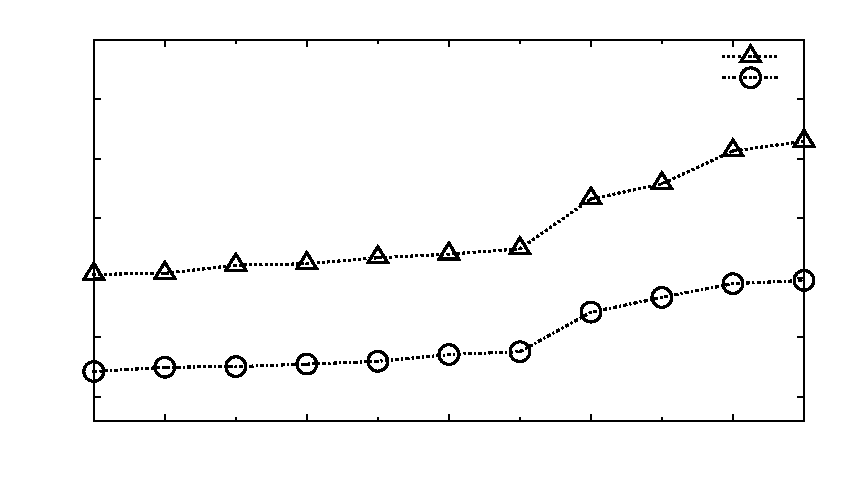
\includegraphics{./plots/plot_weak_scaling}}
      \gplfronttext
    \end{picture}
    \endgroup
  }
  \caption{DD-    $\alpha$    AMG 的弱缩放测试。晶格大小随着进程数量的增加而增加,同时保持每个进程的局部晶格大小固定为    $16 \cdot 8^3$    。  }
  \label{plot:weak_scaling}
\end{figure}

对于扩展研究,我们将粗网格上的迭代次数固定为    $50$    步奇偶预处理 GMRES,以便我们始终具有相同数量的    $100$       \texttt{MPI\_Allreduce}    操作。在图    \ref{plot:weak_scaling}    中,我们看到了通常的    $\mathrm{log}(p)$    依赖性,   $p$    进程数,这是由全局通信引起的,并且从    $512$    到    $1,\!024$    进程时出现了异常增加。其他测量表明,这是由于    \texttt{MPI\_Allreduce}    操作对于    $1,\!024$    处理器需要更长的时间,这是 Juropa 的机器特定功能。除此之外,我们的方法可以很好地扩展到    $8,\!192$    进程。
\subsection{与不精确通缩法的比较  }       \label{ss:leuscher_comp}

\cite{Luescher2007}    的非精确压缩代码已公开发布    \cite{wwwDDHMC}    。现在我们将其性能与 DD-    $\alpha$    AMG 进行比较。   \footnote{根据本文的预印本~   \cite{Frommer:2013fsa}   ,不精确压缩方法已根据 DD-   $\alpha$    AMG 的精神进行了升级(参见~   \cite{wwwOPENQCD}   )。新版本被称为“投影不准确”。我们在此将其与旧的“精确投影”版本进行比较。  }

除了后平滑步骤数    $\nu$    之外,我们选择了两种方法的相同参数。对于不精确压缩方法    $\nu = 5$    和 DD-    $\alpha$    AMG,   $\nu=2$    分别提供了最快的求解器。对于不精确压缩方法,我们使用带有    \texttt{-O3}    标志的    \texttt{gcc}    编译器并手工编码低级    \texttt{SSE}    优化,对于 DD-    $\alpha$    AMG 方法,我们使用带有优化标志    \texttt{-O3 -ipo -axSSE4.2 -m64}    的    \texttt{icc}    编译器。这些编译器选项为相应的代码提供了最佳选择。由于我们的重点是算法改进,因此我们没有针对 DD-    $\alpha$    AMG 进行定制的    \texttt{SSE}    优化,这在原则上应该可以进一步提高速度。以下结果是在与部分~    \ref{ss:setup_eval}    和    \ref{ss:scaling}    相同的    $48^4$    晶格上以及在    $128 \times 64^3$    晶格上产生的(表~    \ref{table:allconfs}    ,id~    \ref{CLS_128_64}    )。

\begin{table}[ht]
  \centering\scalebox{0.9}{\begin{tabular}{ccccccc}
      \toprule
                            & \multicolumn{3}{c}{Inexact deflation} & \multicolumn{3}{c}{DD-        $\alpha$        AMG}                                                                                        \\
      \cmidrule(lr){2-4} \cmidrule(lr){5-7}
      setup                 & setup                                 & iteration                                          & solver          & setup           & iteration                     & solver           \\
      steps         $\ninv$ & timing                                & count (coarse)                                     & timing          & timing          & count (coarse)                & timing           \\
      \midrule
      $ 1 $                 & $1.01$        s                       & $233$                 $(82) $                      & $10.1$        s & $2.08$        s & $149$                 $(24) $ & $ 6.42$        s \\
      $ 2 $                 & $1.87$        s                       & $155$                 $(145)$                      & $10.2$        s & $3.06$        s & $ 59$                 $(46) $ & $ 3.42$        s \\
      $ 3 $                 & $2.69$        s                       & $108$                 $(224)$                      & $9.96$        s & $4.69$        s & $ 35$                 $(63) $ & $ 2.37$        s \\
      $ 4 $                 & $3.43$        s                       & $ 84$                 $(301)$                      & $9.25$        s & $7.39$        s & $ 27$                 $(68) $ & $ 1.95$        s \\
      $ 5 $                 & $6.14$        s                       & $ 70$                 $(320)$                      & $7.50$        s & $10.8$        s & $ 24$                 $(75) $ & $ 1.82$        s \\
      $ 6 $                 & $5.68$        s                       & $ 63$                 $(282)$                      & $5.21$        s & $14.1$        s & $ 23$                 $(84) $ & $ 1.89$        s \\
      $ 8 $                 & $7.71$        s                       & $ 54$                 $(267)$                      & $4.12$        s & $19.5$        s & $ 22$                 $(99) $ & $ 2.02$        s \\
      $10 $                 & $10.1$        s                       & $ 49$                 $(265)$                      & $3.62$        s & $24.3$        s & $ 22$                 $(116)$ & $ 2.31$        s \\
      \bottomrule
    \end{tabular}}
  \caption{比较 DD-    $\alpha$    AMG 与不精确紧缩、粗系统求解器容差    $10^{-12}$    和    $\nu=5$    在    $48^4$    晶格 (表~    \ref{table:allconfs}    : id~    \ref{BMW_48_48}   )、   $2,\!592$    核上的不精确紧缩、病态系统中的差异。  }
  \label{table:DDMLvsID1}
\end{table}

表~    \ref{table:DDMLvsID1}    比较了    $\ninv$    整个范围内的不精确压缩和 DD-    $\alpha$    AMG。我们发现    $\ninv=5$    提供了最快的 DD-    $\alpha$    AMG 求解器,它比需要    $\ninv=10$    的最快不精确压缩求解器快两倍。对于可观测量的计算,如果同一系统需要求解几个右侧,则这两个因素直接影响到总计算时间,因为设置成本可以忽略不计。当查看设置和求解一个右侧的总时间时,   $\ninv=2$    最适合 DD-    $\alpha$    AMG,它需要    $6.48$    秒。不精确压缩的最佳选择是    $\ninv=6$   ,需要    $10.89$    秒。

我们还看到,除了    $\ninv$    的非常小的值之外,DD-   $\alpha$    AMG 中所需的迭代次数还不到不精确紧缩方法中所需迭代次数的一半。括号中的数字表示相应方法每次迭代中粗求解器迭代的平均次数。对于 DD-   $\alpha$    AMG,粗网格上的迭代次数随着设置中花费的工作而增加。因此,最低的 DD-   $\alpha$    AMG 迭代计数并不一定能在双网格设置中提供最快的求解器。在不精确紧缩方法中,粗网格上的迭代次数与    $\ninv$    的联系并不那么明显。由于在不精确紧缩方法中必须非常精确地求解粗系统,因此求解粗网格系统所需的迭代次数高于 DD-   $\alpha$    AMG。但是,它只是适度(高出 2 到 4 倍)而已,因为    \cite{wwwDDHMC}    中的代码在粗系统上的 GCR 迭代中使用了额外的自适应计算预条件器,而我们在 DD-   $\alpha$    AMG 中使用了效率较低的奇偶预条件。

对于相同数量的测试向量,DD-   $\alpha$    AMG 产生的粗系统比不精确压缩系统大两倍(粗网格运算符中包含的非零值是其四倍),但好处是保留了粗网格上的    $\Gamma_5$    结构。DD-   $\alpha$    AMG 粗网格系统似乎更病态——这表明细网格系统的重要方面在粗网格上得到体现——而由此产生的粗网格校正显然更有效地降低了总迭代次数,从而加快了整个方法的速度。

当从二网格转换为多重网格时,病态粗网格系统具有实现大幅改进的潜力。因此,在图    \ref{plot:lvl234}    中,我们报告了使用我们的多重网格代码的实验版本进行的研究结果。它比较了奇偶预处理 BiCGStab 与 DD-    $\alpha$    AMG 的求解器时间,对于不同的质量参数    $m_0$    选择,使用了 2、3 和 4 个级别。从 2 级到 3 级的增益非常明显;对于    $m_0$    的较小值,对应于物理上有趣的状态,我们观察到 2.5 到 3 倍的改进。使用更多级别是不精确通缩代码所不具备的功能。

\begin{figure}[ht]
  \centering\scalebox{0.7}{
    \begingroup
    \makeatletter
    \providecommand\color[2][]{
      \GenericError{(gnuplot) \space\space\space\@spaces}{
        Package color not loaded in conjunction with
        terminal option `colourtext'
      }{See the gnuplot documentation for explanation.
      }{Either use 'blacktext' in gnuplot or load the package
        color.sty in LaTeX.}
      \renewcommand\color[2][]{}
    }
    \providecommand\includegraphics[2][]{
      \GenericError{(gnuplot) \space\space\space\@spaces}{
        Package graphicx or graphics not loaded
      }{See the gnuplot documentation for explanation.
      }{The gnuplot epslatex terminal needs graphicx.sty or graphics.sty.}
      \renewcommand\includegraphics[2][]{}
    }
    \providecommand\rotatebox[2]{#2}
    \@ifundefined{ifGPcolor}{
      \newif\ifGPcolor
      \GPcolorfalse
    }{}
    \@ifundefined{ifGPblacktext}{
      \newif\ifGPblacktext
      \GPblacktexttrue
    }{}
    \let\gplgaddtomacro\g@addto@macro
    \gdef\gplbacktext{}
    \gdef\gplfronttext{}
    \makeatother
    \ifGPblacktext
      \def\colorrgb#1{}
      \def\colorgray#1{}
    \else
      \ifGPcolor
        \def\colorrgb#1{\color[rgb]{#1}}
        \def\colorgray#1{\color[gray]{#1}}
        \expandafter\def\csname LTw\endcsname{\color{white}}
        \expandafter\def\csname LTb\endcsname{\color{black}}
        \expandafter\def\csname LTa\endcsname{\color{black}}
        \expandafter\def\csname LT0\endcsname{\color[rgb]{1,0,0}}
        \expandafter\def\csname LT1\endcsname{\color[rgb]{0,1,0}}
        \expandafter\def\csname LT2\endcsname{\color[rgb]{0,0,1}}
        \expandafter\def\csname LT3\endcsname{\color[rgb]{1,0,1}}
        \expandafter\def\csname LT4\endcsname{\color[rgb]{0,1,1}}
        \expandafter\def\csname LT5\endcsname{\color[rgb]{1,1,0}}
        \expandafter\def\csname LT6\endcsname{\color[rgb]{0,0,0}}
        \expandafter\def\csname LT7\endcsname{\color[rgb]{1,0.3,0}}
        \expandafter\def\csname LT8\endcsname{\color[rgb]{0.5,0.5,0.5}}
      \else
        \def\colorrgb#1{\color{black}}
        \def\colorgray#1{\color[gray]{#1}}
        \expandafter\def\csname LTw\endcsname{\color{white}}
        \expandafter\def\csname LTb\endcsname{\color{black}}
        \expandafter\def\csname LTa\endcsname{\color{black}}
        \expandafter\def\csname LT0\endcsname{\color{black}}
        \expandafter\def\csname LT1\endcsname{\color{black}}
        \expandafter\def\csname LT2\endcsname{\color{black}}
        \expandafter\def\csname LT3\endcsname{\color{black}}
        \expandafter\def\csname LT4\endcsname{\color{black}}
        \expandafter\def\csname LT5\endcsname{\color{black}}
        \expandafter\def\csname LT6\endcsname{\color{black}}
        \expandafter\def\csname LT7\endcsname{\color{black}}
        \expandafter\def\csname LT8\endcsname{\color{black}}
      \fi
    \fi
    \setlength{\unitlength}{0.0500bp}
    \begin{picture}(7920.00,4536.00)
      \gplgaddtomacro\gplbacktext{
        \csname LTb\endcsname
        \put(980,743){\makebox(0,0)[r]{\strut{}        $30$        }}
        \put(980,1032){\makebox(0,0)[r]{\strut{}        $50$        }}
        \put(980,1817){\makebox(0,0)[r]{\strut{}        $200$        }}
        \put(980,2047){\makebox(0,0)[r]{\strut{} }}
        \put(980,2210){\makebox(0,0)[r]{\strut{}        $400$        }}
        \put(980,2336){\makebox(0,0)[r]{\strut{} }}
        \put(980,1425){\makebox(0,0)[r]{\strut{}        $100$        }}
        \put(980,2728){\makebox(0,0)[r]{\strut{}        $1000$        }}
        \put(980,4032){\makebox(0,0)[r]{\strut{}        $10000$        }}
        \put(7075,440){\makebox(0,0){\strut{}        $-0.02$        }}
        \put(6377,440){\makebox(0,0){\strut{}        $-0.03$        }}
        \put(5351,440){\makebox(0,0){\strut{}        $-0.04$        }}
        \put(3383,440){\makebox(0,0){\strut{}        $-0.05$        }}
        \put(2447,440){\makebox(0,0){\strut{}        $m_d$        }}
        \put(2175,440){\makebox(0,0){\strut{} }}
        \put(1865,440){\makebox(0,0){\strut{}        $m_u$        }}
        \put(1359,440){\makebox(0,0){\strut{}        $m_{crit}$        }}
        \put(2175,4335){\makebox(0,0){\strut{}        $m_{ud}$        }}
        \put(160,2387){\rotatebox{-270}{\makebox(0,0){\strut{}time to solution (in seconds)}}}
        \put(4329,140){\makebox(0,0){\strut{}        $m_0$        }}
      }
      \gplgaddtomacro\gplfronttext{
        \csname LTb\endcsname
        \put(6655,3972){\makebox(0,0)[r]{\strut{}inexact deflation}}
        \csname LTb\endcsname
        \put(6655,3772){\makebox(0,0)[r]{\strut{}two-level DD-        $\alpha$        AMG}}
        \csname LTb\endcsname
        \put(6655,3572){\makebox(0,0)[r]{\strut{}three-level DD-        $\alpha$        AMG}}
        \csname LTb\endcsname
        \put(6655,3372){\makebox(0,0)[r]{\strut{}four-level DD-        $\alpha$        AMG}}
        \csname LTb\endcsname
        \put(6655,3172){\makebox(0,0)[r]{\strut{}mp oe BiCGStab}}
      }
      \gplbacktext
      \put(0,0){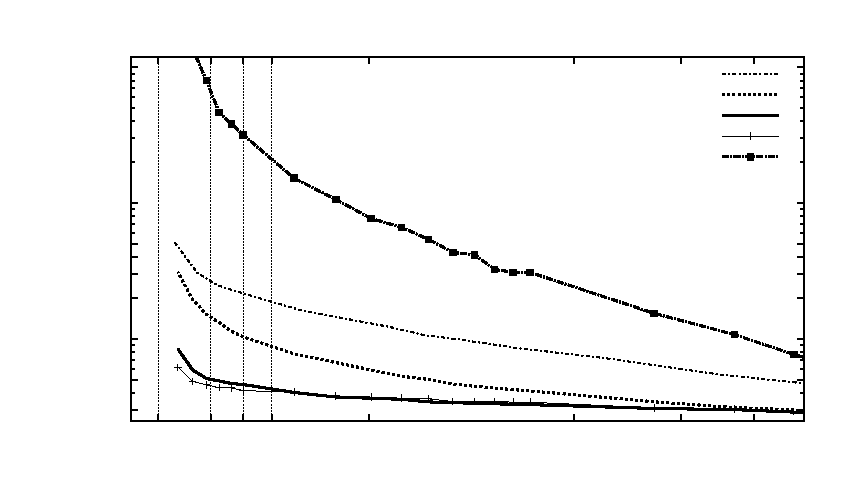
\includegraphics{./plots/plot_3lvl_mass_scaling}}
      \gplfronttext
    \end{picture}
    \endgroup
  }
  \caption{2、3 和 4 级 DD-    $\alpha$    AMG 的质量缩放,
    $64^4$    晶格(表~    \ref{table:allconfs}    :id~    \ref{BMW_64_64}    ),重启长度    $n_{kv}=10$    ,
    $128$    核心。这里,   $m_{ud}$    是平均轻夸克质量(当前大多数模拟都是在此质量及以上进行的),假设上夸克和下夸克具有共同的质量。一些最近的模拟,例如    \cite{Borsanyi:2013lga,Duncan:1996xy,Finkenrath:2013soa}    ,已经区分了上夸克和下夸克的质量,这在不久的将来会变得更加重要。然后接近    $m_u$    的状态变得相关。  }
  \label{plot:lvl234}
\end{figure}

\begin{table}[ht]
  \centering\scalebox{0.9}{\begin{tabular}{lcccc}
      \toprule
                  & Inexact deflation & DD-        $\alpha$        AMG & speed-up factor \\
      \midrule
      smooth iter & $5$               & $2$                            &                 \\
      setup  iter & $5$               & $3$                            &                 \\
      setup  time & $10.9$        s   & $7.85$        s                & $1.39$          \\
      solve  iter & $31$              & $45$                           &                 \\
      solve  time & $8.63$        s   & $5.81$        s                & $1.49$          \\
      total  time & $19.5$        s   & $13.6$        s                & $1.43$          \\
      \bottomrule
    \end{tabular}}
  \caption{对 DD-    $\alpha$    AMG 与    $128 \times 64^3$    晶格(表~    \ref{table:allconfs}   、id~    \ref{CLS_128_64}   )上病态系统上的不精确紧缩进行比较,参数与表~    \ref{table:DDMLvsID1}   、   $8,\!192$    核心中的参数相同。  }
  \label{table:comp_128_64_3}
\end{table}

结束讨论后,我们在表~    \ref{table:comp_128_64_3}    中比较了不精确压缩和 DD-    $\alpha$    AMG,这是许多最近的格点 QCD 计算的典型配置。配置~    \ref{CLS_128_64}    与表~    \ref{table:allconfs}    中的其他配置在生成方式上有所不同,从而产生了完全不同的离散化效果。我们再次采用了默认参数集,但现在设置阶段相对便宜。这导致 DD-    $\alpha$    AMG 中的设置和求解的增益因子超过    $1.4$   ,以对抗不精确压缩。在 DD-    $\alpha$    AMG 中,仍有 55 \% 的执行时间花在粗系统求解上。
\subsection{与 GCR-Smoothing 的比较  }
\label{ss:gmres_smoother}    代数多重网格思想对格点 QCD 系统的普遍适用性首先在~    \cite{MGClark2010_1, MGClark2007, MGClark2010_2}    中被考虑,其中生成的方法被简称为“AMG”,我们将在下文讨论中保留这个术语。该方法已作为 QOPQDP 库的一部分实现,请参阅    \cite{wwwQOPQDP}    ,该库是公开可用的。正如我们在~    \ref{aggregation_based_interpolation_lattice_qcd}    、~    \ref{sec:aAggAMG}    和~    \ref{sec:Boot}    节中所解释的那样,AMG 激发了 DD-    $\alpha$    AMG 中的许多选择,特别是保留    $\Gamma_{5}$    对称性和基于聚合的插值。

这里介绍的方法有两个主要区别。一是平滑迭代的选择。DD-   $\alpha$    AMG 使用 SAP 的某些步骤,可视为“块平滑”,而 AMG 使用“点平滑”,即标准(奇偶预处理)GCR 的某些步骤。另一个重要区别是设置。在    \cite{MGClark2009, MGClark2010_1, MGClark2007, MGClark2010_2}    中考虑了不同的变体,QOPQDP 代码通过将测试向量计算为特征向量的相当精确的近似值来进行。它们是通过应用足够数量的 BiCGStab 迭代一次获得的,同时保持当前向量与所有先前向量正交。

表    \ref{table:comp_amg}    报告了我们两种配置中 DD-    $\alpha$    AMG 与 AMG 的比较。我们将不同的参数选择与 DD-    $\alpha$    AMG 的标准参数设置进行了比较。当初始残差减少    $10^{-5}$    倍(而不是    $10^{-10}$    倍)时,我们停止了迭代,原因是 QOPQDP 配置仅以单精度表示。对于 AMG 中的默认参数选择,我们发现设置成本要高得多(时间上减少 2 到 4 倍),而 DD-    $\alpha$    AMG 每次系统求解的迭代次数略少。我们可以通过减少对每个测试向量 (  {    \em    msi   }  ) 执行的 BiCGStab 迭代的最大次数限制,使 AMG 设置中的工作量与 DD-    $\alpha$    AMG 相当,但随后 AMG 中每次求解的迭代次数会增加,求解时间总是比 DD-    $\alpha$    AMG 更长。域分解平滑器涉及的全局通信比 GCR 少,这对更多核心的求解时间有很大影响。例如,在    $8,\!192$    核心上,求解时间比 AMG 小 2 到 3 倍。

\begin{table}[ht]
  \arraycolsep0.1ex
  \centering\scalebox{0.9}{\begin{tabular}{lccccccc}
      \toprule
                  & \multicolumn{3}{c}{id~\ref{BMW_64_64},         $128$         cores}  & \phantom{m}     & \multicolumn{3}{c}{id~\ref{CLS_128_64},         $256$         cores}                                                                          \\
                  & AMG-d                                                                & AMG-20          & DD-        $\alpha$        AMG                                        &  & AMG-d           & AMG-10          & DD-        $\alpha$        AMG \\
      \midrule
      setup  time & $2424$        s                                                      & $826$        s  & $896$        s                                                        &  & $2464$        s & $607$        s  & $656$        s                 \\
      solve  iter & $14$                                                                 & $22$            & $10$                                                                  &  & $13$            & $21$            & $11$                           \\
      solve  time & $45.4$        s                                                      & $66.0$        s & $57.1$        s                                                       &  & $36.5$        s & $50.4$        s & $37.3$        s                \\
      \midrule
                  & \multicolumn{3}{c}{id~\ref{BMW_64_64},         $8192$         cores} &                 & \multicolumn{3}{c}{id~\ref{CLS_128_64},         $8192$         cores}                                                                         \\
                  & AMG-d                                                                & AMG-40          & DD-        $\alpha$        AMG                                        &  & AMG-d           & AMG-20          & DD-        $\alpha$        AMG \\
      \midrule
      setup  time & $52.3$        s                                                      & $24.6$        s & $27.7$        s                                                       &  & $89.9$        s & $29.1$        s & $32.3$        s                \\
      solve  iter & $14$                                                                 & $16$            & $10$                                                                  &  & $13$            & $16$            & $11$                           \\
      solve  time & $4.75$        s                                                      & $5.51$        s & $1.82$        s                                                       &  & $3.49$        s & $3.43$        s & $1.86$        s                \\
      \bottomrule
    \end{tabular}}
  \caption{DD-    $\alpha$    AMG 和 AMG 的比较。AMG-d 使用默认参数设置,AMG-    $k$    设置    $ msi  = k$   ,因此设置时间与 DD-    $\alpha$    AMG 相当。AMG 中的    \texttt{SSE}    优化已关闭。  }
  \label{table:comp_amg}
\end{table}

\section\*{致谢  }    我们感谢两位匿名审稿人提出的几条宝贵建议。我们还感谢布达佩斯-马赛-伍珀塔尔合作组织为 Juropa 提供配置和计算时间。我们还要感谢 James Brannick(宾夕法尼亚州立大学)就多重网格方法的开发提供的建议、Kalman Szab  { 韓國   } (伍珀塔尔贝尔吉斯大学)对实施的支持、Wolfgang S  { 韓國   }  ldner(雷根斯堡大学)对 I/O 接口的帮助以及 Norbert Eicker(伍珀塔尔贝尔吉斯大学和 JSC)分享他在 Juropa 方面的专业知识。

\bibliographystyle{siam}
\begin{thebibliography}{10}

  \bibitem{Alexandrou:2011db}
  {\sc C.~Alexandrou, M.~Brinet, J.~Carbonell, M.~Constantinou, P.~A. Harraud,
    P.~Guichon, K.~Jansen, T.~Korzec, and M.~Papinutto}, {\em Nucleon
      electromagnetic form factors in twisted mass lattice {QCD}}, Phys. Rev.,
  D83:094502 (2011).

  \bibitem{Aoki:2008sm}
  {\sc S.~Aoki, K.-I. Ishikawa, N.~Ishizuka, T.~Izubuchi, D.~Kadoh, K.~Kanaya,
    Y.~Kuramashi, Y.~Namekawa, M.~Okawa, Y.~Taniguchi, A.~Ukawa, N.~Ukita, and
    T.~Yoshie}, {\em 2+1 flavor lattice {QCD} toward the physical point}, Phys.
  Rev., D79:034503 (2009).

  \bibitem{MGClark2009}
  {\sc R.~Babich, J.~Brannick, R.~C. Brower, M.~A. Clark, S.~D. Cohen, J.~C.
    Osborn, and C.~Rebbi}, {\em The role of multigrid algorithms for {LQCD}},
  PoS, LATTICE2009:031 (2009).

  \bibitem{MGClark2010_1}
  {\sc R.~Babich, J.~Brannick, R.~C. Brower, M.~A. Clark, T.~A. Manteuffel, S.~F.
    McCormick, J.~C. Osborn, and C.~Rebbi}, {\em Adaptive multigrid algorithm for
  the lattice {W}ilson-{D}irac operator}, Phys. Rev. Lett., 105:201602 (2010).

  \bibitem{Bae:2011ff}
  {\sc T.~Bae, Y.-C. Jang, C.~Jung, H.-J. Kim, J.~Kim, K.~Kim, W.~Lee, S.~R.
    Sharpe, and B.~Yoon}, {\em Kaon {        $B$        }-parameter from improved staggered
      fermions in         $n_f=2+1$         {QCD}}, Phys. Rev. Lett., 109:041601 (2012).

  \bibitem{Bali:2012qs}
  {\sc G.~S. Bali, P.~C. Bruns, S.~Collins, M.~Deka, B.~Gl{\"{a}}{\ss}le,
  M.~G{\"{o}}ckeler, L.~Greil, T.~R. Hemmert, R.~Horsley, J.~Najjar, Y.~Nakamura,
  A.~Nobile, D.~Pleiter, P.~E.~L. Rakow, A.~Sch{\"{a}}fer, R.~Schiel,
  G.~Schierholz, A.~Sternbeck, and J.~Zanotti}, {\em Nucleon mass and sigma
      term from lattice {QCD} with two light fermion flavors}, Nucl. Phys., B866
  (2013), pp.~1--25.

  \bibitem{Banks:1979yr}
  {\sc T.~Banks and A.~Casher}, {\em Chiral symmetry breaking in confining
      theories}, Nucl.Phys., B169 (1980), p.~103.

  \bibitem{Ben-Av:1990gb}
  {\sc R.~Ben-Av, M.~Harmatz, S.~Solomon, and P.~G. Lauwers}, {\em Fermion
      simulations using parallel transported multigrid}, Phys. Lett., B253 (1991),
  pp.~185--192.

  \bibitem{PRACE:ScAnnRep12}
  {\sc T.~Bergrath, M.~Ramalho, R.~Kenway, et~al.}, {\em {PRACE} scientific
      annual report 2012}, tech. report, PRACE, 2012.
  \newblock
  \texttt{http://www.prace-ri.eu/IMG/pdf/PRACE\_Scientific\_Annual\_Report\_2012.pdf},
  p.~32.

  \bibitem{Borsanyi:2013lga}
  {\sc S.~Borsanyi, S.~D{\"{u}}rr, Z.~Fodor, J.~Frison, C.~Hoelbling, S.~D. Katz,
  S.~Krieg, T.~Kurth, L.~Lellouch, T.~Lippert, A.~Portelli, A.~Ramos,
  A.~Sastre, and K.~K. Szabo}, {\em Isospin splittings in the light baryon
      octet from lattice {QCD} and {QED}},  (2013).

  \bibitem{DBraess_1995}
  {\sc D.~Braess}, {\em Towards algebraic multigrid for elliptic problems of
      second order}, {Computing}, {55} ({1995}), pp.~379--393.

  \bibitem{brandt2002}
  {\sc A.~Brandt}, {\em Multiscale scientific computation: Review 2001}, in
  Multiscale and Multiresolution Methods, T.~J. Barth, T.~Chan, and R.~Haimes,
  eds., vol.~20 of Lecture Notes in Computational Science and Engineering,
  Springer Berlin Heidelberg, 2002, pp.~3--95.

  \bibitem{KahlBootstrap}
  {\sc A.~Brandt, J.~Brannick, K.~Kahl, and I.~Livshits}, {\em Bootstrap {AMG}},
  SIAM J. Sci. Comput., 33 (2011), pp.~612--632.

  \bibitem{MGClark2007}
  {\sc J.~Brannick, R.~C. Brower, M.~A. Clark, J.~C. Osborn, and C.~Rebbi}, {\em
      Adaptive multigrid algorithm for lattice {QCD}}, Phys. Rev. Lett., 100:041601
  (2007).

  \bibitem{Brezina2005}
  {\sc M.~Brezina, R.~Falgout, S.~MacLachlan, T.~Manteuffel, S.~McCormick, and
    J.~Ruge}, {\em Adaptive smoothed aggregation {(        $\alpha$        SA)} multigrid}, SIAM
  Review, 47 (2005), pp.~317--346.

  \bibitem{Sanders10}
  {\sc M.~Brezina, T.~Manteuffel, S.~McCormick, J.~Ruge, and G.~Sanders}, {\em
      Towards adaptive smoothed aggregation {(        $\alpha$        SA)} for nonsymmetric
      systems}, SIAM J. Sci. \  Comput., 32 (2010), pp.~14--39.

  \bibitem{Brower:1987dd}
  {\sc R.~Brower, E.~Myers, C.~Rebbi, and K.~Moriarty}, {\em The multigrid method
      for fermion calculations in quantum chromodynamics}, Tech. Report
  Print-87-0335, IAS,Princeton, 1987.

  \bibitem{wwwCLS}
  {\sc CLS}, {\em Coordinated lattice simulation}.
  \newblock \texttt{https://twiki.cern.ch/twiki/bin/view/CLS/}.

  \bibitem{DeGrand:2006zz}
  {\sc T.~DeGrand and C.~E. Detar}, {\em Lattice Methods for Quantum
      Chromodynamics}, World Scientific, 2006.

  \bibitem{Degrand1990211}
  {\sc T.~A. DeGrand and P.~Rossi}, {\em Conditioning techniques for dynamical
      fermions}, Comput. Phys. Commun., 60 (1990), pp.~211--214.

  \bibitem{Duncan:1996xy}
  {\sc A.~Duncan, E.~Eichten, and H.~Thacker}, {\em Electromagnetic splittings
      and light quark masses in lattice {QCD}}, Phys. Rev. Lett., 76 (1996),
  pp.~3894--3897.

  \bibitem{Durr21112008}
  {\sc S.~D{\"{u}}rr, Z.~Fodor, J.~Frison, C.~Hoelbling, R.~Hoffmann, S.~D. Katz,
  S.~Krieg, T.~Kurth, L.~Lellouch, T.~Lippert, K.~Szabo, and G.~Vulvert}, {\em
      Ab initio determination of light hadron masses}, Science, 322 (2008),
  pp.~1224--1227.

  \bibitem{Durr:2010aw}
  {\sc S.~D{\"{u}}rr, Z.~Fodor, C.~Hoelbling, S.~D. Katz, S.~Krieg, et~al.}, {\em
      Lattice {QCD} at the physical point: Simulation and analysis details}, JHEP,
  08(2011)148 (2011).

  \bibitem{BMW1}
  {\sc S.~D{\"{u}}rr, Z.~Fodor, C.~Hoelbling, S.~D. Katz, S.~Krieg, T.~Kurth,
  L.~Lellouch, T.~Lippert, K.~K. Szabo, and G.~Vulvert}, {\em Lattice {QCD} at
      the physical point: Light quark masses}, Phys. Lett. B701,  (2011),
  pp.~265--268.

  \bibitem{Finkenrath:2013soa}
  {\sc J.~Finkenrath, F.~Knechtli, and B.~Leder}, {\em One flavor mass
      reweighting in lattice {QCD}}, Nucl. Phys., B877 (2013), pp.~441--456.

  \bibitem{Fritzsch:2012wq}
  {\sc P.~Fritzsch, F.~Knechtli, B.~Leder, M.~Marinkovic, S.~Schaefer, R.~Sommer,
    and F.~Virotta}, {\em The strange quark mass and {Lambda} parameter of two
      flavor {QCD}}, Nucl. Phys., B865 (2012), pp.~397--429.

  \bibitem{Frommer:2013fsa}
  {\sc A.~Frommer, K.~Kahl, S.~Krieg, B.~Leder, and M.~Rottmann}, {\em Adaptive
  aggregation based domain decomposition multigrid for the lattice {W}ilson
  {D}irac operator}, arXiv:1303.1377,  (2013).

  \bibitem{Nobile2012}
  {\sc A.~Frommer, A.~Nobile, and P.~Zingler}, {\em Deflation and flexible
        {SAP}-preconditioning of {GMRES} in lattice {QCD} simulation}, tech. report,
  2012.
  \newblock arXiv:1204.5463 [hep-lat].

  \bibitem{Gattringer:2010zz}
  {\sc C.~Gattringer and C.~B. Lang}, {\em Quantum Chromodynamics on the
      Lattice}, vol.~788 of Lect. Notes Phys., Springer, 1st~ed., 2009.

  \bibitem{Gohberg_etal_2005}
  {\sc I.~Gohberg, P.~Lancaster, and L.~Rodman}, {\em Indefinite Linear Algebra
      and Applications}, Birkh{\"{a}}user, Basel, 2005.

  \bibitem{PRACE:ScC12}
  {\sc M.~Guest, G.~Aloisio, R.~Kenway, et~al.}, {\em The scientific case for
        {HPC} in {E}urope 2012 - 2020}, tech. report, PRACE, October 2012.
  \newblock \texttt{http://www.prace-ri.eu/PRACE-The-Scientific-Case-for-HPC},
  p.~75.

  \bibitem{hackbusch2003multi}
  {\sc W.~Hackbusch}, {\em Multi-Grid Methods and Applications}, vol.~4 of
  Springer Series in Computational Mathematics, Springer, 1st~ed., 2003.

  \bibitem{Kahl-Rittich-preprint}
  {\sc K.~Kahl and H.~Rittich}, {\em Analysis of the deflated conjugate gradient
      method based on symmetric multigrid theory}.
  \newblock Preprint BUW-IMACM 12/19, 2012.

  \bibitem{Kalkreuter:1994fz}
  {\sc T.~Kalkreuter}, {\em Multigrid methods for propagators in lattice gauge
      theories}, J. Comput. Appl. Math., 63 (1995), pp.~57--68.

  \bibitem{Kennedy:2006ax}
  {\sc A.~D. Kennedy}, {\em Algorithms for dynamical fermions},
  arXiv:hep-lat/0607038,  (2006).

  \bibitem{Krieg:2010zz}
  {\sc S.~Krieg and T.~Lippert}, {\em Tuning lattice {QCD} to petascale on {B}lue
  {G}ene/{P}}, {NIC} {S}ymposium 2010,  (2010), pp.~155--164.

  \bibitem{Lippert19991357}
  {\sc T.~Lippert}, {\em Parallel {SSOR} preconditioning for lattice {QCD}},
  Parallel Computing, 25 (1999), pp.~1357--1370.

  \bibitem{wwwDDHMC}
  {\sc M.~L{\"{u}}scher}, {\em {DD-HMC} algorithm for two-flavour lattice {QCD}}.
  \newblock \texttt{http://luscher.web.cern.ch/luscher/DD-HMC}, used version:
  {DD-HMC}-1.2.2, September 2008.

  \bibitem{wwwOPENQCD}
  {\sc M.~L{\"{u}}scher}, {\em {openQCD} simulation program for lattice {QCD} with
      open boundary conditions}.
  \newblock \texttt{http://luscher.web.cern.ch/luscher/openQCD/}, used version:
  {openQCD}-1.2, May 2013.

  \bibitem{Luescher2003}
  \leavevmode\vrule height 2pt depth -1.6pt width 23pt, {\em Solution of the
        {D}irac equation in lattice {QCD} using a domain decomposition method},
  Comput. Phys. Commun. 156,  (2004), pp.~209--220.

  \bibitem{Luescher2007}
  \leavevmode\vrule height 2pt depth -1.6pt width 23pt, {\em Local coherence and
      deflation of the low quark modes in lattice {QCD}}, JHEP, 07(2007)081 (2007).

  \bibitem{montvay1994quantum}
  {\sc I.~Montvay and G.~M{\"{u}}nster}, {\em Quantum Fields on a Lattice},
  Cambridge Monographs on Mathematical Physics, Cambridge University Press,
  1994.

  \bibitem{wwwQOPQDP}
  {\sc J.~C. Osborn}, {\em Multigrid solver for clover fermions, implementation
      within {QOPQDP}}.
  \newblock \texttt{http://usqcd.jlab.org/usqcd-docs/qopqdp/}, used version:
  QOPQDP 0.19.0, April 2013.

  \bibitem{MGClark2010_2}
  {\sc J.~C. Osborn, R.~Babich, J.~Brannick, R.~C. Brower, M.~A. Clark, S.~D.
    Cohen, and C.~Rebbi}, {\em Multigrid solver for clover fermions}, PoS,
  LATTICE2010:037 (2010).

  \bibitem{Rittich2011}
  {\sc H.~Rittich}, {\em Deflation in multigrid methods}, master's thesis,
  Bergische Universtit{\"{a}}t Wuppertal, 2011.

  \bibitem{RugeStueben87}
  {\sc J.~Ruge and K.~St{\"{u}}ben}, {\em Algebraic multigrid}, in Multigrid
  Methods, S.~F. McCormick, ed., vol.~3 of Frontiers in Applied Mathematics,
  SIAM, Philadelphia, 1987, pp.~73--130.

  \bibitem{Saad:2003:IMS:829576}
  {\sc Y.~Saad}, {\em Iterative Methods for Sparse Linear Systems}, SIAM,
  Philadelphia, PA, USA, 2nd~ed., 2003.

  \bibitem{Schwarz1870}
  {\sc H.~Schwarz}, {\em Gesammelte mathematische {A}bhandlungen},
  Vierteljahrschrift Naturforsch. Ges. Z{\"{u}}rich,  (1870), pp.~272--286.

  \bibitem{Sheikholeslami:1985ij}
  {\sc B.~Sheikholeslami and R.~Wohlert}, {\em Improved continuum limit lattice
      action for {QCD} with {W}ilson fermions}, Nucl. Phys., B259 (1985),
  pp.~572--597.

  \bibitem{SiSz03}
  {\sc V.~Simoncini and D.~B. Szyld}, {\em Theory of inexact {K}rylov subspace
      methods and applications to scientific computing}, SIAM J. Sci. Comput., 25
  (2003), pp.~454--477.

  \bibitem{BFSmith_PEBjorstad_WDGropp_1996a}
  {\sc B.~F. Smith, P.~E. Bj{\o}rstad, and W.~D. Gropp}, {\em Domain
      Decomposition: Parallel Multilevel Methods for Elliptic Partial Differential
      Equations}, Cambridge University Press, New York, 1996.

  \bibitem{smith1985numerical}
  {\sc G.~Smith}, {\em Numerical Solution of Partial Differential Equations:
      Finite Difference Methods}, Oxford Applied Mathematics and Computing Science
  Series, Clarendon Press, 1985.

  \bibitem{Tang:2010:CTP:1958286.1958296}
  {\sc J.~M. Tang, S.~P. MacLachlan, R.~Nabben, and C.~Vuik}, {\em A comparison
      of two-level preconditioners based on multigrid and deflation}, SIAM J.
  Matrix Anal. Appl., 31 (2010), pp.~1715--1739.

  \bibitem{UTrottenberg_etal_2001}
  {\sc U.~Trottenberg, C.~W. Oosterlee, and A.~Sch{\"{u}}ller}, {\em Multigrid.
  With Guest Contributions by A. Brandt, P. Oswald, K. St{\"{u}}ben}, Academic
  Press, Orlando, FL, 2001.

  \bibitem{EshofSlei04}
  {\sc J.~van~den Eshof and G.~L. Sleijpen}, {\em Inexact {K}rylov subspace
      methods for linear systems}, SIAM J. Matrix Anal. Appl., 26 (2004),
  pp.~125--153.

  \bibitem{Vink:1991fa}
  {\sc J.~C. Vink}, {\em Multigrid inversion of staggered and {W}ilson fermion
      operators with {        $SU(2)$        } gauge fields in two-dimensions}, Phys. Lett., B272
  (1991), pp.~81--85.

  \bibitem{Wilson:1975id}
  {\sc K.~G. Wilson}, {\em Quarks and strings on a lattice}, in New Phenomena in
  Subnuclear Physics. Part A. Proceedings of the First Half of the 1975
  International School of Subnuclear Physics, Erice, Sicily, July 11 - August
  1, 1975, A.~Zichichi, ed., vol.~321 of {CLNS} Reports, New York, 1977, Plenum
  Press.

\end{thebibliography}



\end{document}



